%%%%%%%%%%%%%%%%%%%%%%%%%%%%%%%%%%%%%%%%%%%%%%%%
\input{./format/preamble.ltx} 
%%%%%%%%%%%%%%%%%%%%%%%%%%%%%%%%%%%%%%%%%%%%%%%%
% as needed, comment the following lines by prefixing the percent sign (%) at the start of the line

% Drafttrue % comment to disable putting some guides in the draft form of the document

\PutLineNumberstrue % comment to disable line numbers and certain  preparation guides 

\Figurestrue % comment to disable the rendering figures

\GroupIDtrue % comment to disable group ID

\ResultDiscusstrue % comment to disable results and discussions

\Conctrue % comment to disable conclusions

% todo: comment or uncomment this to see the acknowledgment part
\Finishedtrue % comment to disable manuscript for final defense or binding/submission
% todo: replace the thesis approval sheet with the signed one
% \ApprovalSheetSignedtrue % comment to disable inclusion of the signed approval sheet

%\Gradtrue % comment to disable graduate school format

%\PhDtrue % comment to disable PhD dissertation format

%\PubListtrue % comment to disable publication list

% \Vitatrue % comment to disable author(s) vita

\Indextrue % comment to disable index 

%%%%%%%%%%%%%%%%%%%%%%%%%%%%%%%%%%%%%%%%%%%%%%%%
% document IDs

% specify if dissertation, thesis, project, dissertation proposal, thesis proposal, project proposal 
%\newcommand{\documentType}{Thesis} 
\newcommand{\documentType}{Thesis}
%\newcommand{\documentType}{Dissertation Proposal}
%\newcommand{\documentType}{Dissertation}
\newcommand{\college}{Gokongwei College of Engineering}
\newcommand{\department}{Department of Electronics and Computer Engineering} 
\newcommand{\degreeType}{Bachelor of Science}
%\newcommand{\degreeType}{Bachelor and Master of Science}  
%\newcommand{\degreeType}{Master of Engineering Program} 
%\newcommand{\degreeType}{Master of Science} 
%\newcommand{\degreeType}{Doctor of Philosophy} 
\newcommand{\degree}{Computer Engineering}
\newcommand{\degreeAbbrv}{BS-CPE}
%\newcommand{\degreeAbbrv}{BS-MS-ECE}
%\newcommand{\degreeAbbrv}{MEP-ECE}
%\newcommand{\degreeAbbrv}{MS-ECE}
%\newcommand{\degreeAbbrv}{PhD-ECE}

\newcommand{\documentAdviserTitle}{Dr.} 
\newcommand{\documentAdviser}{Reggie C. Gustilo}

\newcommand{\examinerChairTitle}{Dr.} 
\newcommand{\examinerChair}{Donabel de Veas Abuan}

% Sort in alphabetically ascending manner the surnames of the examiners
\newcommand{\examinerATitle}{Dr.} 
\newcommand{\examinerA}{Ronnel P. Agulto}

\newcommand{\examinerBTitle}{Dr.} 
\newcommand{\examinerB}{Alexander Co Abad}

% Note that \examinerC and \examinerD only applies for PhD dissertations
% \newcommand{\examinerCTitle}{Dr.} 
% \newcommand{\examinerC}{Rafael W. Sison}

% \newcommand{\examinerDTitle}{Dr.} 
% \newcommand{\examinerD}{Apolinario V. Valenzuela}

% College signatories for graduate theses/dissertations
% \newcommand{\RASDTitle}{Dr.} 
% \newcommand{\RASDName}{Isabella S. Garcia}

% \newcommand{\deanTitle}{Dr.} 
% \newcommand{\deanName}{Diego U. Lopez}

\newcommand{\groupID}{AISL-1-2425-C5} % group ID is for undergraduates as of this formatting

\newcommand{\numberOfAuthors}{4} % adapt the number of names below accordingly and sort the sunames in alphabetically ascending manner, like in the following example

\defineAuthor{surname1}{Banal}
\defineAuthor{firstname1}{Kenan A.}

\defineAuthor{surname2}{BAUTISTA}
\defineAuthor{firstname2}{Francis Robert Miguel F.}

\defineAuthor{surname3}{HERMOSURA}
\defineAuthor{firstname3}{Don Humphrey L.}

\defineAuthor{surname4}{SALAZAR}
\defineAuthor{firstname4}{Daniel G.}

\newcommand{\documentTitle}{Non-Destructive Carabao Mango Sorter and Grader based on Physical Characteristics using Machine Learning} % put tilde (~) between words to indicate non-breaking adjacent words

\newcommand{\keywords}{\glspl{machine learning}, \gls{Carabao mango}, \glspl{bruises}, \glspl{ripeness}, \glspl{microcontroller}}

\newcommand{\finalDefenseDate}{\usdate\today} % replace ''\usdate\today'' by your final defense date; you may need to use non-breaking space with the use of tildes (~); if so, do not remove the tildes in order to not break the date

\ifGrad
\newcommand{\scannedApprovalSheetFileName}{./figure/Signed_Thesis_Approval_Sheet_Graduate.pdf} % filename of the signed approval sheet (for graduate)
\else	
\newcommand{\scannedApprovalSheetFileName}{./figure/Signed_Thesis_Approval_Sheet_Undergraduate.pdf} % filename of the signed approval sheet (for undergraduate)
\fi

\hyphenation{op-tical net-works semi-conduc-tor evi-dent re-la-tive re-si-den-tial po-la-ri-za-tion so-lu-tion/s} % for correcting bad hyphenation

%%%%%%%%%%%%%%%%%%%%%%%%%%%%%%%%%%%%%%%%%%%%%%%%
\input{./format/postamble.ltx} 

%%%%%%%%%%%%%%%%%%%%%%%%%%%%%%%%%%%%%%%%%%%%%%%%
% for placing user-defined-ambles

\DeclareMathAlphabet{\mathitbf}{OML}{cmm}{b}{it} % for math italic bold, but can also use \mathbfit
\newcommand{\redtx}[1]{\textcolor[rgb]{0.65,0.16,0}{#1}} % for formatting text to have a red color
\newcommand{\graytx}[1]{\textcolor[rgb]{0.75,0.75,0.75}{#1}} % for formatting text to have a gray color

%%%%%%%%%%%%%%%%%%%%%%%%%%%%%%%%%%%%%%%%%%%%%%%%
% \includeonly{} is for specifying which files to include; if you only want to work on one or few chapters, you can only include those chapters, which will speed up the document build; advantage: fast if you have a large number of images in your results chapter, which you do not need when you are working on other chapters; you can still reference all the figures in the omitted chapter, as long as you have previously LaTeX-built the entire document

% Note that the file names below must correspond to those names inside \include{} in the \begin{document} ... \end{doument} enviroment, otherwise the chapter will not be included

%  the excludeonly package provides the logically opposite command: \excludeonly{<file list>}

\includeonly{% just comment those portions that you do not want to be included in the parsing
	introduction,
	literature_review,
	theoretical_considerations,
	design_considerations,
	methodology,
	results_and_discussions,
	conclusions,
	answers_to_questions,
	revisions_to_the_proposal,
	revisions_to_the_final,
	usage_examples,
	publication,
	vita,
}

%%%%%%%%%%%%%%%%%%%%%%%%%%%%%%%%%%%%%%%%%%%%%%%%
\begin{document}
	\pagenumbering{roman} % roman page numbering starts here
	
	%%%%%%%%%%%%%%%%%%%%%%%%%%%%%%%%%%%%%%%%%%%%%%%%
	\input{./format/pre_toc.ltx}
	\cleardoublepage
	
	%%%%%%%%%%%%%%%%%%%%%%%%%%%%%%%%%%%%%%%%%%%%%%%%
	\begin{SingleSpace}
		\tableofcontents
		\cleardoublepage
		
		%%%%%%%%%%%%%%%%%%%%%%%%%%%%%%%%%%%%%%%%%%%%%%%%
		\listoffigures
		\cleardoublepage
		
		%%%%%%%%%%%%%%%%%%%%%%%%%%%%%%%%%%%%%%%%%%%%%%%%
		\listoftables
		\cleardoublepage
		
		%%%%%%%%%%%%%%%%%%%%%%%%%%%%%%%%%%%%%%%%%%%%%%%
		\phantomsection
		\addcontentsline{toc}{chapter}{Abbreviations and Acronyms}
		{
			\printterms[database=abbreviation, style=indexalign, prelocation=dotfill, location=first, columns=1, postname=\hspace{3em}]
			\thispagestyle{plain}
		}	
		\cleardoublepage
		
		%%%%%%%%%%%%%%%%%%%%%%%%%%%%%%%%%%%%%%%%%%%%%%%
		\phantomsection
		\addcontentsline{toc}{chapter}{Notations}
		{
			\printterms[database=notation, style=indexalign, prelocation=dotfill, location=first, columns=1, postname=\hspace{3em}]
			
			\thispagestyle{plain}
		}
		\cleardoublepage
		
		%%%%%%%%%%%%%%%%%%%%%%%%%%%%%%%%%%%%%%%%%%%%%%%%
		\phantomsection
		\addcontentsline{toc}{chapter}{Glossary}
		{
			\printterms[database=glossary, style=indexalign, prelocation=none, location=hide, columns=1, postname=\hspace{3em}]
			\thispagestyle{plain}
		}
		\cleardoublepage
		
		%%%%%%%%%%%%%%%%%%%%%%%%%%%%%%%%%%%%%%%%%%%%%%%%
		\lstlistoflistings
		\cleardoublepage
	\end{SingleSpace}
	
	%%%%%%%%%%%%%%%%%%%%%%%%%%%%%%%%%%%%%%%%%%%%%%%%
	\pagenumbering{arabic} % arabic page numbering starts here
	\chapter{Introduction}
	\label{ch:intro}
	%\startcontents[chapters]
	%\begin{SingleSpace}	
	%	\Mprintcontents  % for creating an actual mini TOC for this chapter
	%\end{SingleSpace}
	\section{Background of the Study}

Mangoes, also known as the Mangifera indica, are a member of the cashew family. 
This fruit can often be seen being farmed by countries such as Myanmar, the Philippines, 
and India as they have a tropical dry season. Being in a tropical country is an important 
aspect for mango cultivation as it ensures proper growth for mangoes. 
If aspects such as temperature and rainfall are not ideal, it may affect the quality 
of the mango \citep{noauthor-mango-2024}. 
Carabao mangoes is a variety of a mango that is found and cultivated in the
Philippines. It is known for its sweet signature taste that was recognized
sweetest in the world in the Guinness Book of World Records in 1995. The mango
was named after the national animal of the Philippines, a native breed of
buffalo. On average, it is 12.5 cm in length and 8.5 cm in diameter, having a
bright yellow color when ripe as seen in Figure \ref{fig:img1}. It is often cultivated
during late May to early July \citep{DBpediaCarabao}.

\begin{figure}[!htbp]
	\centering
	\includegraphics[width=0.5\textwidth]{fig1}
	\caption{Carabao Mangoes at Different Ripeness Stages \citep{guillermo-determining-2019}}
	\label{fig:img1}
\end{figure}

Likewise, the Philippines produced an estimated 596.34 thousand metric tons of mangoes 
during the April-June 2023 quarter, marking an 11.4 percent 
increase from the 535.43 thousand metric tons harvested in the same three-month period of 
2022. Of this total output, the Carabao mango variety accounted for the vast 
majority at 495.06 thousand metric tons, or 83.0 percent of the nation's entire mango production \citep{psa2023major}.

This shows that mangoes are a highly valued fruit in the Philippines as
it is not only the country’s national fruit but also amongst the leading
agricultural exports of the country, ranking only third below bananas and
pineapples. This gives the country the 9th slot amongst the leading exporters of
Mangoes across the world. Attributed to this ranking is the country's export of
both fresh and dried mangoes, as well as low tariff rates. This allows the
country to export a large quantity of the fruit in countries such as Singapore,
Japan, and the USA as they can enter duty free markets provided by the World
Trade Organization and Japan. Due to this, the mangoes have become a major
source of income to an estimated 2.5 million farmers in the country
\citep{centino-current-nodate}.

Before mangoes are sold in markets, they first undergo multiple post-harvest
processes. This is to ensure that the mangoes that arrive in markets are utmost
quality before being sold to consumers. Moreover, it ensures that mangoes are
contained and preserved properly such that they do not incur damages and/or get
spoiled on its transportation to the market. Processing of the mango involves
pre-cooling, cleaning, waxing, classification, grading, ripening, packaging,
preservation, storage, packing, and transportation \citep{patel-novel-2019}
\citep{rizwan-iqbal-classification-2022}.

Among the processes that mangoes undergo, classification and grading is
important as it allows the manufacturer to separate mangoes with good qualities
versus mangoes with poor qualities. According to a study by
\citep{lacap-bruise-2021}, size, length, width, volume, density, indention, and
grooves are aspects that determine the maturity of mangoes. These traits are
being checked along with the ripeness of the mango, sightings of bruise injury,
and cracks on the fruit \citep{lacap-bruise-2021} as these aspects affect the
sellability of the fruit as well as the chances of it getting spoiled sooner.

Previous studies have been made to automate the sortation process of the
mangoes. Among these is a research done by \citet{abbas-mango-2018}, which
focuses on classification of mangoes using their texture and shape features.
They do this by, first, acquiring an image of the mango using a digital camera.
Then, these images are fed to the MaZda package, which is a software originally
developed for magnetic resonance imaging. Within the MaZda package is the B11
program, which uses Principal Component Analysis, Linear Discriminant Analysis,
Nonlinear Discriminant Analysis, and texture classification to extract features
from the mango, which in this case are the length, width, and texture. This data
is then compared to a database in order to classify any given mango
\citep{abbas-mango-2018}.  

Another study is done by \citet{rizwan-iqbal-classification-2022}, which
classifies mangoes based on their color, volume, size, and shape This is done by
making use of Charge Coupled Devices, Complementary Metal-Oxide Semiconductor
sensors, and 3-layer \gls{Convolutional Neural Network}. To classify the mangoes,
images are first captured and preprocessed to be used as a data set
\citep{rizwan-iqbal-classification-2022}. This data set is then augmented to be
used as a model for the 3-layer \gls{Convolutional Neural Network}. After extracting
the features of the mango, the 3-layer \gls{Convolutional Neural Network} is used as a
method for their classification as it can mimic the human brain in pattern
recognition, and process data for decision making. This is important as some
mangoes have very subtle differences which make it difficult to differentiate
them.



\section{Prior Studies}

A paper written by \citet{amna-et-al-machine-2023}, designed an automated fruit
sorting machine based on the quality through 
an image acquisition system and \acr{CNN}. Furthermore, the results of the paper show
that the image processing detection score was 89\% while that of the tomatoes
was 92\% while the CNN model had higher validity of 95\% for mangoes and 93\% 
for tomatoes. 15\%, while the percentage of distinction between the two groups
was reported to be 5\% respectively 
\citep{amna-et-al-machine-2023}. Despite the high \gls{accuracy score}  in
detecting mango defects, the fruit sorting system only sorts based 
on the mango defects and not on ripeness, and weight.

Furthermore, the research paper presented by \citet{guillergan-naive-2024}
designed an Automated Carabao mango classifier, in which the mango image
database is used to extract the features like size, area along with the ratio of
the spots for grading using Naïve Bayes Model. For the results, the Naïve Bayes’
model recognized large and rejected mangoes with 95\% accuracy and the large and
small/medium difference with a 7\% error, suggesting an application for quality
differentiation and sorting in the mango business industry. Despite the high
accuracy of classifying Carabao mangoes, the researchers used a high quality
DSLR camera for the image acquisition system without any \gls{microcontroller}
to control the mangoes \citep{guillergan-naive-2024}. 


\section{Problem Statement}
As mangoes are among the top exports of the Philippines
\citep{centino-current-nodate}, assessing the physical deformities is a
necessity. The physical deformities of the Carabao mango can determine the
global competitiveness of the country. Having higher quality exports can often
lead to gaining competitive edge, increase in demand, increase export revenues,
and becoming less susceptible to low-wage competition
\citep{dadamo-determinants-2018}. In order to increase the quality of mango
fruit exports, a key post-harvest process is done, which is sorting and grading.
Mango sorting and grading then becomes important to determine which batches are
of high quality and can be sold for a higher price, and which batches are of low
quality and can only be sold for a low price
\citep{zhengzhou-first-industry-co-ltd-what-nodate}. Traditionally, fruit
sorting and grading is inefficient as it is done manually by hand. Some tools
are used such as porous ruler to determine fruit size and color palette for
color grading \citep{zhengzhou-first-industry-co-ltd-what-nodate}. However,
among the problems encountered in the process of manually sorting and grading
mangoes are susceptibility to human error and requiring a number of laborers to
do the task. 

With the current advancements in technology, some researchers have already taken
steps to automate the process of sorting and grading mangoes. However, these
attempts would often only consider some of the aspects pertaining to size,
ripeness, and \gls{bruises} but not dynamically change the method of sorting and grading.
Furthermore, most of the research papers have a fix static method in grading and sorting the mangoes.
This means that it doesn't take into consideration the user's priority when grading and
sorting the mangoes. Lastly, not
all research approaches were able to implement a hardware for their algorithm,
limiting their output to only a software implementation and not an embedded
system. As such the proposed system would assess the quality of the
Carabao mango based on all the mentioned mango traits, namely size,
\gls{bruises}, and ripeness while also taking into consideration being
non-destructive and the user's priority when grading and sorting the mangoes.
These aspects are important because, as was previously
mentioned, there is a need to develop a user priority based Carabao mango sorter that 
takes into
account all these aspects at the same time while being non-destructive.



\section{Objectives and Deliverables}

\subsection{General Objective (GO)}
\begin{itemize}
	\item \Copy{GO}{GO: To develop a user-priority-based grading and sorting system for Carabao mangoes, 
		using \gls{machine learning} and \gls{computer vision} techniques to assess ripeness, size, and bruises. };
\end{itemize}

\subsection{Specific Objectives (SOs)}

\begin{itemize}
	\item \Copy{SO1}{SO1: To make an image acquisition system with a conveyor belt for 
		automatic sorting and grading mangoes. };
	
	\item \Copy{SO2}{SO2: To get the precision, recall, F1 score, confusion matrix,
		and train and test accuracy metrics for classifying the ripeness and bruises with an accuracy score of at least 90\%.};
	
	\item \Copy{SO3}{SO3: To create a microcontroller-based system to operate the image acquisition system, 
		control the conveyor belt, and process the mango images through machine learning. };
	
	\item \Copy{SO4}{SO4: To grade mangoes based on user priorities for size, ripeness, and bruises.  };
	
	\item \Copy{SO5}{SO5: To classify mango ripeness based on image data using machine learning algorithms
		such as kNN, k-mean, and Naïve Bayes.  };
	
	\item \Copy{SO6}{SO6: To classify mango size based on image data by getting its length and width using OpenCV, 
		geometry, and image processing techniques. };
	
	\item \Copy{SO7}{SO7: To classify mango bruises based on image data by employing machine learning algorithms.}
\end{itemize}



\subsection{Expected Deliverables}

Table~\ref{tab:expected_deliverables} shows the outputs, 
products, results, achievements, gains, realizations, and/or
yields of the \documentType. 

\begin{center}
	{\scriptsize
		\begin{longtable}{p{0.3\textwidth}|p{0.6\textwidth}}
			\caption{Expected Deliverables per Objective} \label{tab:expected_deliverables} \\
			\hline 
			\hline 
			\textbf{Objectives} & 
			\textbf{Expected Deliverables} \\ 
			\hline 
			\endhead
			\hline 
			\multicolumn{2}{r}{\textit{Continued on next page}} \\ 
			\endfoot
			\hline 
			\endlastfoot
			\hline
			\Paste{GO} & \begin{itemize}
				\item To develop a Carabao mango grading and sorting system.
				\item To grade Carabao mangoes into three categories based on ripeness, size, and 
				bruises using machine learning.
				\item To integrate sensors and actuators to control the conveyor belt and image acquisition system.
			\end{itemize} \\ \hline
			
			\Paste{SO1} & \begin{itemize}
				\item To make an image acquisition system with a camera and LED light source.
				\item To build a flat belt conveyor for moving the mangoes.
			\end{itemize} \\ \hline
			
			\Paste{SO2} & \begin{itemize}
				\item To use a publicly available dataset of at least 10,000 mango images
				for classification of ripeness and bruises.
			\end{itemize} \\ \hline
			
			\Paste{SO3} & \begin{itemize}
				\item To develop an intuitive UI where users can start and stop the system.
				\item To implement a priority-based grading system with sliders for ripeness, bruises, and size.
			\end{itemize} \\ \hline
			
			\Paste{SO4} & \begin{itemize}
				\item To utilize a linear combination formula as the overall mango score, where each classification level 
				contributes a grade, weighted by the priority assigned to the three properties.
				\item To assign score values for each classification level of the mango.
			\end{itemize} \\ \hline
			
			\Paste{SO5} & \begin{itemize}
				\item To train a machine learning model such as kNN, k-means, or Naïve Bayes capable
				of classifying mango ripeness based on the image color.
				\item To gather a dataset of annotated images with ripeness labels.
				\item To obtain an evaluation report of performance metrics of the model.
			\end{itemize} \\ \hline
			
			\Paste{SO6} & \begin{itemize}
				\item To develop an image processing algorithm capable of determining mango 
				size using OpenCV, NumPy, and imutils.
				\item To classify mangoes based on size into small, medium, and large based on measurements.
			\end{itemize} \\ \hline
			
			\Paste{SO7} & \begin{itemize}
				\item To train a machine learning model such as 
				CNN capable of distinguishing bruised and non-bruised mangoes.
				\item To train a machine learning model such as kNN, k-means, and Naïve Bayes 
				capable of assessing the extent of bruising on the mangoes if it is significant or partial.
				\item To gather a dataset of annotated images based on bruises.
				\item To obtain an evaluation report of performance metrics of both CNN and other machine learning models.
			\end{itemize} \\ \hline
			
		\end{longtable}
	}
\end{center}


\section{Significance of the Study}

Automating the process of sorting and grading mangoes increases efficiency and
productivity for the user which would in effect remove human error in sorting
and grading and decrease the human labor and time taken to sort and grade the
mangoes.  This is especially important for farmers with a large amount of fruit
such as mangoes and a lesser labor force. A recent study showed that their
automated citrus sorter and grader using computer vision can reduce the human
labor cost and time to sort and grade when comparing the automated citrus sorter
and grader to manual human labor \cite{chakraborty-development-2023}. 

Another benefit to automating sorting and grading mangoes is the improvement in
quality control.  This implies that compared to human labor, automating sorting
and grading mangoes can uniformly assess the quality of mangoes based on size,
color, and \gls{bruises}, ensuring that the expected grade and high-quality
mangoes reach the consumer. By accurately identifying substandard mangoes, the
system helps in reducing waste and ensuring that only marketable fruits are
processed further.

Likewise, the scalability of automating sorting and grading mangoes is simpler,
especially for lower labor force farmers with large volumes of mangoes. Because
of the possibility of large-scale operations by automating sorting and grading
mangoes, farmers can now handle large volumes of mangoes, making them suitable
for commercial farms and processing plants. Moreover, it can be adapted to
different varieties of mangoes and potentially other fruits with minor
modifications.


\subsection{Technical Benefit}

\begin{enumerate}
	\item The development of an automated \gls{Carabao mango} sorter would increase the quality control 
	of classifying \gls{Carabao mango} based on ripeness, size, and bruising.
	
	\item The accuracy in sorting Carabao mangoes will be significantly improved while
	reducing the errors due to human factors in manual sorting.
	
	\item The automated \gls{Carabao mango}  sorter carefully sorts the mangoes 
	while ensuring that they remain free from bruising or further damage during the process	
\end{enumerate}

\subsection{Social Impact}

\begin{enumerate}
	\item The reduction in manual labor creates opportunities in maintenance and
	technologies in the automated \gls{Carabao mango}  sorter.
	
	\item The automated \gls{Carabao mango}  sorter system improves Carabao mango 
	standards and enhances the satisfaction of the buyers and the customers through
	guaranteeing consistent Carabao mango grade.
	
	\item Opportunity to increase sales and profit for the farmers through consistent 
	quality and grade Carabao mangoes while reducing the physical labor to sort it.
\end{enumerate}

\subsection{Environmental Welfare}

\begin{enumerate}
	\item With the utilization of non-destruction methods of classifying Carabao mangoes together with an
	accurate sorting system, overall waste from Carabao mangoes is reduced and the likelihood
	of improperly sorted mangoes is decreased.
	
	\item Automation of sorting and grading Carabao mangoes promotes sustainable farming practices.
	
\end{enumerate}



\section{Assumptions, Scope, and Delimitations}

\subsection{Assumptions}

\begin{enumerate}
	\item The Carabao mangoes are from the same source together with the same variation
	
	\item The Carabao mangoes do not have any fruit borer and diseases
	
	\item All the components do not have any form of defects
	\item The prototype would have access to constant electricity/power source.
	\item The Carabao mangoes to be tested would be in the post-harvesting stage and in the grading stage.
	\item The image-capturing system would only capture the two sides of the mango which 
	are the two largest surface areas of the skin.	
\end{enumerate}

\subsection{Scope}
\begin{enumerate}
	\item The prototype would be specifically designed to grade and 
	sort Carabao Mangoes based on only ripeness, size, and visible skin bruises.
	
	\item The mangoes used as the subject will be solely sourced from markets in the Philippines.
	
	\item The Carabao mangoes would be graded into three levels.
	\item The prototype will be using a microcontroller-based system locally stored on 
	the device itself to handle user interaction.
	\item Computer vision algorithms to be used will include image classification.
\end{enumerate}

\subsection{Delimitations}
\begin{enumerate}
	\item The project would only be able to perform sorting and grading on one specific fruit 
	which is the Carabao mango and will not be able to sort other types of mangoes.
	
	\item Additionally, the project prototype will only be able to capture, sort, and grade one 
	mango subject at a time which means the mangoes have to be placed in the conveyor belt in
	a single file line for accurate sorting. 
	
	\item For the bruises, the system will only be able to detect external bruises and 
	may not identify the non-visible and internal bruises.
	\item The system does not load the mangoes onto the conveyor belt itself. 
	Assistance is required to put mangoes into the conveyor belt to start the sorting process
	\item The prototype will be powered using \acr{AC} power and will be plugged into 
	a wall socket which is only suitable for indoor use.
\end{enumerate}


\ifFinished
\else

\section{Estimated Work Schedule and Budget}

\begin{figure}[!htbp]
	\centering
	\includegraphics[width=1\textwidth]{ganttchart}
	\caption{Gantt Chart}
	\label{fig:img2}
\end{figure}

As seen above, Table~\ref{fig:img2} shows the Gantt Chart together with the
assigned task. For the first part of the THSCP4A, the group would primarily
revise and fine tune Chapters 1 and 2 while also preparing for the defense.
After that for THSCP4B, the yellow team which consists of two members, Hermosura
and Salazar, would start buying and collecting the materials needed for
assembling the prototype. While team yellow is doing that, team purple which
consists of Banal and Baustista would start training and validating the
\acr{CNN} model based on the Carabao mango image dataset. After that integration
of the sensors and actuators together with the integration of the \acr{CNN}
model and beginning of coding of the Application to the \acr{RPi} would be
done. Once that \acr{CNN} model is deployed and the Application works testing of
the Carabao mangoes to the prototype would be done. During THSCP4C, data
gathering would be done together with polishing and revising of the final paper.

\ifPhD
\section{Publication Plan}
\graytx{\blindtext}
\fi

\fi


\section{Overview of the \documentType}

There are seven succeeding chapters. To recall, chapter 1 involves the
introduction of the thesis topic containing the background of the study,
previous studies, objectives and deliverables, assumptions, scope, and
delimitation, significance of the study, description of the project together
with the methodology, and Gantt chart and budget. Chapter 2 involves the
existing articles, the lacking in their approaches, and the summary of chapter
2. Chapter 3 involves the theoretical considerations of the thesis topic while
chapter 4 would consist of the design consideration involving the thesis topic.
Chapter 5 would involve the research methodology containing the testing
procedure and setup.  Chapter 6 would involve the results and discussion based
on the methodology while Chapter 7 would involve the conclusion,
recommendations, and future suggestions.

	%\stopcontents[chapters]
	\cleardoublepage
	
	%%%%%%%%%%%%%%%%%%%%%%%%%%%%%%%%%%%%%%%%%%%%%%%%
	\chapter{Literature Review} 
	\label{ch:litrev} 
	%\startcontents[chapters]
	%\begin{SingleSpace}	
	%	\Mprintcontents 
	%\end{SingleSpace}
	

\section{Existing Work}

The research paper written by \citet{adam-non-destructive-2022} developed a ripeness grader for
Carabao mangoes. The Carabao mango ripeness grade calculated based on object and
color detection which were written in microcontroller. These are the systems designed
by the researchers that consists of Raspberry Pi 4, Arduino Uno, camera, touch screen
LCD, MQ3 gas sensor, ventilation system. The proposed system was able to ascertain an
overall reliability of 95\%: therefore, the specified objective of ascertaining the ripeness
level of the mangoes was met with success. However, accuracy and reliability of the
software system are there since the hardware design does not seem to be workable when
one must deal with the scores of mangoes \citep{adam-non-destructive-2022}. In addition, the design of the hardware does
not integrate any form of physical automating, say like the conveyor belt. Besides, the
hardware system only works efficiently when deciding the ripeness grade of mangoes
separately.

A study done by \citet{school-of-engineering-asia-pacific-college-philippines-carabao-2023} is another research paper that supports and has
relevant information concerning the topic. The researchers proposed a fully-perovskite
photonic system which has the capability to identify and sort or grade mango based on
features such as color, weight and, conversely, signs of damages \citep{school-of-engineering-asia-pacific-college-philippines-carabao-2023}. Some of the techniques
in image processing that the researchers used included image enhancement, image
deblurring, edge detection using MATLAB and Arduino as well as color image
segmentation. By carrying out the multiple trials on the device they achieved a
classification speed of 8.132 seconds and an accuracy of 91.2\%. The proponents’
metrics used for the ratings were speed wherein the results were rated “excellent” while
the accuracy rating given was “good”. One of the limitations of the paper is that the
researchers were only limited to the color, texture, and size of the Carabao mango

Furthermore, the research paper presented by \citet{guillergan-naive-2024} designed an
Automated Carabao mango classifier, in which the mango image database is used to
extract the features like weight, size, area along with the ratio of the spots for grading
using Naïve Bayes Model. Concerning the quantitative test design, one had to control
and experiment with various methods of image processing that would improve the
likelihood of improved classification. The paper methodology entailed sample collection
from 300 Carabao mangoes, picture taking using a DSLR camera, and feature
deconstruction for categorization \citep{guillergan-naive-2024}. The system prototype and
the software were designed with the programming language C\# with integration of
Aforge. NET routines. The performance of this model was checked with the help of the
dataset containing 250 images, precision, recall, F-score key indicators were used. The
investigation discovered that the Naïve Bayes’ model recognized large and rejected
mangoes with 95\% accuracy and the large and small/medium difference with a 7\% error,
suggesting an application for quality differentiation and sorting in the mango business
industry. The limitations in the researchers’ paper include the researchers were able to
achieve high accuracy after using a high quality DSLR camera and the fact that the
researchers were not able to incorporate the use of microcontrollers.

Another study by \citet{tomas-detection-2022} proposed SVM-based system for classifying the maturity stages of bananas, mangoes, and calamansi. With the use of 1729 images of bananas together with 711 mango images and 589 calamansi, the researchers were able to achieve a high accuracy score of above 90\% for all fruits. Some pre-processing techniques used to get this high accuracy are the change in hue, saturation, and value channels in the mango image \citep{tomas-detection-2022}. To better understand the harvest time of mangoes, the paper by \citet{abu-determination-2021} examined the association of the harvest season with seasonal heat units, rainfall, and physical fruit attributes for Haden, Kent, Palmer, and Keitt mango varieties to establish export and domestic market maturity standards. For the results of the paper, it shows that temperature, rainfall, and physical characteristics have a reliable, non-destructive indicators for determining mango maturity \citep{abu-determination-2021}. This shows that physical characteristics and temperature are important when exporting fruits such as mangoes.


\begin{table}[h]
	\centering
	\caption{Comparison of Existing Studies}
	\label{tab:comparison_existing_studies}
	\renewcommand{\arraystretch}{1.3}
	\begin{tabular}{p{0.2\textwidth}|p{0.6\textwidth}|p{0.1\textwidth}}
		\hline
		\textbf{Existing Study} & \textbf{Limitations} & \textbf{Accuracy Rating} \\
		\hline
		\citet{adam-non-destructive-2022} & No physical automation, not suitable for large amounts of mangoes, only classifies ripeness and only a sample size of 10 mangoes. & 95\% \\
		\hline
		\citet{school-of-engineering-asia-pacific-college-philippines-carabao-2023} & Focuses only on color and size. & 91.2\% \\
		\hline
		\cite{guillergan-naive-2024} & Relies on high-quality DSLR cameras, and limited automation due to not integrating microcontrollers. & 95\% \\
		\hline
		\citet{supekar-multi-parameter-2020} & No physical automation implemented. Ripeness, size, and shape-based classification achieved 100\%, 98.19\%, and 99.20\% accuracy respectively on their own. However, errors occurred when taking into account all these aspects together for grading mangoes, causing an accuracy rating deduction. & 88.88\% \\
		\hline
	\end{tabular}
\end{table}

Previous studies on mango grading have achieved an accuracy rating of up to 95\%, as
shown in Table~\ref{tab:comparison_existing_studies}. However, these studies either relied on a small sample size, which
limits statistical significance, or utilized expensive equipment, which may be
impractical. In light of this, the researchers have set a target accuracy rating of greater than or equal to 90\%.
This target ensures that the system being developed is comparable to, or better than,
existing studies that used larger sample sizes or assessed multiple mango traits at the
same time. Furthermore, this research aims to distinguish itself by not only maintaining
or exceeding the 90\% accuracy rating but also incorporating a graphical user interface
(GUI) for selective priority-based mango classification. The system will integrate both
software and hardware components, and it will evaluate a greater number of mango
traits for grading purposes.

\subsection{Sorting Algorithms}
In previous studies, researchers have implemented various artificial intelligence
algorithms in order to determine the optimal and most effective method for sorting
mangoes. One of the algorithms that was used in the classification of mangoes was the
CNN or Convolutional Neural Networks. A study done by \citet{zheng-mango-2021}
explored the effectiveness of CNN, specifically in classifying mangoes through image
processing. The system that the researchers developed graded mangoes into four groups
which was based on the Chinese National Standard \citep{zheng-mango-2021}. These mangoes were examined by
their shape, color uniformity, and external defects. The system that was developed had
an impressive accuracy of 97.37\% in correctly classifying the mangoes into these
grading categories
Support Vector Machine was also one of the classification algorithms that was
implemented to detect flaws in mangoes. In that study by \citet{veling-mango-2019}, SVM
was used in the classification of diseases from mangoes. The study used 4 different
diseases/defects for testing \citep{veling-mango-2019}. The diseases were Anthracnose, Powdery Mildew, Black
Banded, and Red Rust. and provided 90\% accuracy for both the leaves and the fruit

In the study done by \citet{schulze-development-2015}, Simple
Linear Regression, Multiple Linear Regression, and Artificial Neural Network models
were all studied and compared for the purpose of size-mass estimation for mango fruits.
The researchers found that the Artificial Neural Network yielded a high accuracy rating
for mass estimation and for mango classification based on size with a success rate of
96.7\% \citep{schulze-development-2015}. This is attributed to the Artificial Neural Network model’s ability to learn both
linear and nonlinear relationships between the inputs and the outputs. However, a
problem can occur with the use of the model, which is overfitting. This issue occurs
when the model is overtrained with the data set such that it will start to recognize
unnecessary details such as image noise which results in poor generalization when fed
with new data. With this in mind, additional steps will be necessary to mitigate the issue.
Another research article written by \citet{alejandro-grading-2018}
implements a method for sorting and grading Carabao mangoes. This research focuses
on the use of Probabilistic Neural Network, which is another algorithm that is used for
pattern recognition and classification of objects. For this study, the researchers focused
on the area, color, and the black spots of the mango for their Probabilistic Neural
Network model \citep{alejandro-grading-2018}. Their research using the model yielded an accuracy rating of 87.5\% for
classification of the mangoes which means it is quite accurate for classifying mangoes
within the predefined categories. However, problems were encountered with the use of
the model when trying to identify mangoes that did not fit the predefined size categories
of small, medium, and large. This means that the PNN model may become challenged
when presented with a mango with outlying traits or traits that were very different from
the data set.

\begin{table}[h]
	\centering
	\caption{Comparison of Sorting Algorithm Models}
	\label{tab:sorting_algorithm_models}
	\renewcommand{\arraystretch}{1.3} % Adjust row spacing
	\begin{tabular}{p{0.3\textwidth}|p{0.1\textwidth}|p{0.2\textwidth}|p{0.3\textwidth}}
		\hline
		\textbf{Sorting Algorithm Model} & \textbf{Accuracy Rating} & \textbf{Criteria} & \textbf{Problems Encountered} \\
		\hline
		Convolution Neural Network & 97.37\% & shape, color, defects & Minor blemishes affected the accuracy. \\
		\hline
		Support Vector Machine & 90\% & mango defects and diseases & The model is sensitive to noise, which requires intensive image preprocessing. \\
		\hline
		Artificial Neural Network & 96.7\% & for mango size and mass & Overfitting \\
		\hline
		Probabilistic Neural Network & 87.5\% & for mango area, color, and black spots & Difficulty in identifying mangoes that have outlying features or did not fit the predefined 		categories \\
		\hline
	\end{tabular}
\end{table}

\section{Lacking in the Approaches}

The majority of past researchers such as \citet{amna-et-al-machine-2023} and \citet{guillermo-determining-2019} were able to implement a fruit and mango sorter together with an accurate AI
algorithm to detect the ripeness defects. This means that none of the previous research
papers were able to integrate an interchangeable user-priority-based grading together
with size, ripeness, and bruises using machine learning for Carabao mango sorter and
grader. Our research however would implement an automated Carabao mango sorter in
terms of size, ripeness, and bruises with its own UI, conveyor belt, stepper motors, and
bins for collecting the different ripeness and defect grade of the Carabao mango.

\section{Summary}

To reiterate, there is an innovative gap that needs to be filled with regards to the process
of sorting and grading Carabao mangoes. The traditional methods for conducting this
process manually by hand, by a porous ruler, by a sugar meter, and by a color palette can
be prone to human error and expensive costs due to the number of laborers required to
do the task. On the other hand, although researchers have already taken steps to
automate the process of mango sorting and grading, there is still a need for an
implementation that takes into account size, ripeness, and bruises altogether whilst being
non-destructive and having its own embedded system. The research articles shown
above show the different computer vision and CNN approaches for sorting and
classifying mangoes. For example, a system created by \citet{adam-non-destructive-2022} was more
focused on ripeness detection. \citet{school-of-engineering-asia-pacific-college-philippines-carabao-2023} considered photonic systems for
grading mango fruit based on color and weight. On the other hand, \citet{guillermo-determining-2019} implemented the Naïve Bayes classification model on mangoes with high
accuracy, which thereby did not include any microcontroller. There was an attempt to
study each of those parameters separately and that is why the multifactorial approach
was not used. With this in mind, the system being proposed does exactly what was
mentioned, to implement a non-destructive and automated sorting and grading system
for Carabao mangoes that takes into account size, ripeness, and bruises altogether using
machine learning, as well as having its own embedded system. This system will be
mainly composed of a conveyor belt, servo motors, a camera, microcontrollers, and an
LCD display for the user interface. By doing so, the system should be able to improve
the efficiency and productivity of mango sorting and grading, remove the effect of
human error and reduce time consumption. The studies also provided critical insights
regarding the effective algorithms that can be used in classification stages in image
processing. The use of CNN had the most accuracy with manageable potential
challenges. Lastly, by scaling the implementation, the overall export quality of the
Carabao mangoes can be improved.





	%\stopcontents[chapters]
	\cleardoublepage
	
	%%%%%%%%%%%%%%%%%%%%%%%%%%%%%%%%%%%%%%%%%%%%%%%%
	\chapter{Theoretical Considerations}
	%\chaptermark{Theoretical Considerations} % uncomment this and put a shorter version of the chapter title for the TOC and chapter markings (i.e., header or footer)
	\label{ch:theorycon}
	%\startcontents[chapters]
	%\begin{SingleSpace}	
	%	\Mprintcontents 
	%\end{SingleSpace}
	

\section{Introduction}

Likewise, the purpose of this chapter is to go through the important theories in developing the prototype together with training and testing the machine learning model.

\section{Relevant Theories and Models}

\begin{figure}[!htbp]
	\centering
	\includegraphics[width=0.5\textwidth]{theoreticalDiagram1}
	\caption{Theoretical Framework Diagram.}
	\label{fig:theoreticalDiagram1}
\end{figure}


The theoretical framework seen in figure x revolves around the concepts that revolve around the research topic. Embedded systems include the Raspberry Pi, which is the microcontroller that will be the brain of the system, DC motors, 4 channel relays, and the conveyor belt. The machine learning portion includes a neural network model, namely the Convolutional Neural Network, which will use computer vision as a method of seeing and classifying the mangoes based on their physical traits. The image processing will include methods such as size calculation and background removal using OpenCV. Lastly, the Carabao mango will be the test subject of the system.

\section{Technical Background}

At its core, the system will be using machine learning concepts pertaining to CNN and OpenCV, and may use other algorithms such as Naive Bayes and k-Nearest Neighbors to supplement the classification tasks, particularly for assessing mango ripeness, bruise detection, and size determination. The system will be built on an embedded framework, integrating a Raspberry Pi microcontroller to control the RaspberryPi camera, actuators, LED lights, and motors. A user-friendly GUI will also be utilized to ensure users can customize the prioritization of the mango sorting system.

\section{Conceptual Framework Background}


\begin{figure}[!htbp]
	\centering
	\includegraphics[width=0.5\textwidth]{theoreticalDiagram2}
	\caption{Conceptual Framework Diagram.}
	\label{fig:theoreticalDiagram2}
\end{figure}


\section{Summary}

Overall, chapter 3 establishes key concepts and theoretical considerations that form the foundation of the Carabao mango sorter and grading system. It discusses and connects each component together, explaining how each component such as the RaspberryPi and DC motors work together to create a system that utilizes machine learning and computer vision techniques to classify mangoes based on user priority.
	%\stopcontents[chapters]
	\cleardoublepage
	
	%%%%%%%%%%%%%%%%%%%%%%%%%%%%%%%%%%%%%%%%%%%%%%%%
	\chapter{Design Considerations} 
	\label{ch:designcon} 
	%\startcontents[chapters]
	%\begin{SingleSpace}	
	%	\Mprintcontents 
	%\end{SingleSpace}
	
Likewise, the objective of chapter 4 is to describe the researcher's design 
consideration when developing and testing the prototype. For an overview of 
the design of the prototype, the researchers considered different computer vision models in
 classifying the ripeness and bruises together with other algorithms to determine 
 the size of the mango. Likewise, the hardware design was also taken into consideration where 
 the physical design of the conveyor belt was taken into account.

\section{Introduction}
This chapter discusses the design considerations for the mango 
sorting and grading system, focusing on the technical and engineering decisions 
required for its development. The design process aims to create a scalable, efficient, 
and user-friendly system that leverages machine learning for accurate mango classification.

\section{System Architecture}
The system architecture is represented through a block diagram, showcasing modules such as image acquisition, 
preprocessing, feature extraction, machine learning model, and grading output. Each module is described in detail, 
emphasizing its role in the overall system. For instance, the image acquisition module uses high-resolution cameras 
to capture mango images, while the preprocessing module enhances image quality for better feature extraction.

\section{Hardware Considerations}
The hardware components include high-resolution cameras, lighting systems for consistent image capture, and 
microcontrollers like Raspberry Pi or Arduino for system control, actuators like DC and stepper motors to move 
the mangoes. The choice of hardware is justified based on cost, performance, and compatibility with the software framework.

\subsection{General Prototype Framework}

\subsection{Prototype Block Diagram}

\subsection{Prototype Flowchart}

\subsection{Hardware Specifications}

\subsubsection{Raspberry Pi}
\begin{figure}[!htbp]
	\centering
	\includegraphics[width=0.5\textwidth]{rpi4b}
	\caption{Raspberry Pi 4 Model B}
	\label{fig:rpi4b_fig}
\end{figure}
The Raspberry Pi 4 Model B is a compact, low-cost computer that serves as the system's main processing unit. 
It was chosen for its balance of performance and affordability, making it suitable for image processing tasks.
Furthermore, it was selected for its compatibility with various peripherals through the GPIO pins and USB-A ports together
with its ease of integration into the prototype.
\\
\\
\textbf{Specifications:}
\begin{itemize}
    \item SoC: Broadcom BCM2711
    \item CPU: Quad-core ARM Cortex-A72 (64-bit)
    \item Clock Speed: 1.5 GHz (base, overclockable)
    \item RAM: 8GB LPDDR4-3200 SDRAM
    \item Wireless: Dual-band 2.4 GHz / 5 GHz Wi-Fi (802.11ac)
    \item Bluetooth: Bluetooth 5.0 (BLE support)
    \item Ethernet: Gigabit Ethernet (full throughput)
    \item USB: 2 x USB 3.0 ports and 2 x USB 2.0 ports
    \item Video Output: 2 x micro-HDMI ports (supports 4K @ 60Hz, dual 4K display capability)
    \item Audio: 3.5mm audio/video composite jack
    \item Storage: MicroSD card slot (supports booting via SD card or USB)
    \item GPIO: 40-pin GPIO header (backward-compatible with older models)
    \item Camera/Display: CSI (camera) and DSI (display) ports
    \item Power Input: USB-C (5V/3A recommended)
    \item Power Consumption: ~3W idle, up to 7.5W under load
\end{itemize}

\subsubsection{Raspberry Pi Camera}
\begin{figure}[!htbp]
	\centering
	\includegraphics[width=0.5\textwidth]{rpi_cam}
	\caption{Raspberry Pi Camera Module Version 2}
	\label{fig:rpi_cam_fig}
\end{figure}
The Raspberry Pi Camera Module Version 2 is a high-quality camera module designed for the Raspberry Pi platform.
Likewise, it is capable of capturing still images at 8 megapixels, and supports video recording at 1080p @ 30fps, 
720p @ 60fps, and 480p @ 90fps. 
Moreover, it has a fixed-focus lens with a diagonal field of view of 62.2 degrees, and an optical format of 1/4 inch. 
Furthermore, it supports various Python libraries such as Picamera and OpenCV for image capture and processing.
As such, it was selected for its compact size, ease of integration, and ability to capture high-resolution images. 
\\
\\
\textbf{Specifications:}
\begin{itemize}
    \item Sensor: Sony IMX219PQ 8-megapixel CMOS sensor.
    \item Still Images Resolution: 8 MP (3280 x 2464 pixels).
    \item Video Resolution: Supports up to 1080p @ 30fps, 720p @ 60fps, and 480p @ 90fps.
    \item Focus: Fixed-focus lens (manual focus adjustment not supported without physical modification).
    \item Lens Size: 1/4-inch optical format.
    \item Field of View (FoV): Diagonal 62.2 degrees.
    \item Interface: Connected via 15-pin ribbon cable to the Raspberry Pi's CSI (Camera Serial Interface) port.
    \item APIs/Libraries: Supports Python libraries such as Picamera and OpenCV for image capture and processing.
    \item Dimensions: 25 mm x 24 mm x 9 mm.
\end{itemize}

\subsubsection{DC Motor}
\begin{figure}[!htbp]
	\centering
	\includegraphics[width=0.5\textwidth]{dc_motor}
	\caption{12 Volt DC Gear Motor}
	\label{fig:dc_motor_fig}
\end{figure}
The 12 Volt DC Gear Motor is a compact, high-torque, and low-noise motor suitable for a 
wide range of applications, including robotics, automation, and industrial control systems. 
It features a spur gear design, which provides a high reduction ratio for increased torque output. 
The motor is designed for continuous operation and has a low power consumption under standard load 
conditions. Likewise, it is also capable of withstanding high temperatures and has a high reliability.
This motor was selected for its high torque output, low power consumption, and compact size, 
making it ideal for the conveyor system.
\\
\\
\textbf{Specifications:}
\begin{itemize}
    \item Gearbox Type: Spur gear design
    \item Operating Voltage: 12V (operational range: 6-12V)
    \item No-load Current Consumption: 0.8A
    \item Rated Current Draw: 3A (under standard load)
    \item No-load Speed: 282 RPM (maximum)
    \item Operating Speed: 248 RPM (under rated load)
    \item Torque Output: 18 kg-cm (rated)
    \item Stall Torque: 60 kg-cm (maximum)
    \item Power Rating: 50W (maximum)
    \item Unit Weight: 350 grams
\end{itemize}


\subsubsection{MicroSD Card}
\begin{figure}[!htbp]
	\centering
	\includegraphics[width=0.5\textwidth]{sdCard}
	\caption{SanDisk Ultra MicroSD Card}
	\label{fig:sdCard_fig}
\end{figure}
The SanDisk Ultra MicroSD Card is a compact, high-capacity, and secure digital memory card 
that is suitable for a wide range of applications, including digital cameras, smartphones, and tablets.
It features a high-speed data transfer rate, making it ideal for storing large files such as images and videos.
This card was selected for its high capacity, secure data protection, and ease of use,
making it ideal for the storage system for the prototype. 
\\
\\
\textbf{Specifications:}
\begin{itemize}
    \item Capacity: 256GB
    \item Type: MicroSDXC (Secure Digital eXtended Capacity)
    \item Form Factor: MicroSD (11mm x 15mm x 1mm)
    \item File System: Pre-formatted exFAT
\end{itemize}

\subsubsection{LED Lights}
\begin{figure}[!htbp]
	\centering
	\includegraphics[width=0.5\textwidth]{led}
	\caption{LED Light Strip}
	\label{fig:led_fig}
\end{figure}
For the \gls{LED}, they were used to provide consistent lighting for image capture, ensuring accurate color representation and feature extraction.
The LED lights were selected for their energy efficiency, long lifespan, and ability to produce a uniform light output.
\\
\\
\textbf{Specifications:}
\begin{itemize}
    \item Power Input: 5V DC (USB-powered, compatible with laptops, power banks, or USB adapters).
    \item Waterproof Design: Suitable for indoor/outdoor use.
    \item LED Type: SMD 2835 (surface-mount diodes for high brightness and efficiency).
    \item Color Type: White (cool white)
    \item Length: 1m 
    \item Beam Angle: 120°
    \item Operating Temperature: -25°C to 60°C.
    \item Storage Temperature: -40°C to 80°C.
\end{itemize}


\subsubsection{Power Supply}
\begin{figure}[!htbp]
	\centering
	\includegraphics[width=0.5\textwidth]{Power_Supply}
	\caption{Bench Power Supply}
	\label{fig:Power_Supply_fig}
\end{figure}
The bench power supply is a versatile and adjustable power source used to 
provide stable voltage and current for various electronic projects.
It is designed for testing applications, allowing users to set specific voltage and current levels.
This power supply was selected for its versatility, 
ease of use, and ability to provide accurate voltage and current control for the prototype.
\\
\\
\textbf{Specifications:}
\begin{itemize}
    \item Type: SMPS (Switch-Mode Power Supply)
    \item Input: 110V AC, 50/60Hz (U.S. Standard)
    \item Output Range: 0-30V DC / 0-5A DC
    \item Voltage Precision: ±0.010V (10 mV) resolution
    \item Current Precision: ±0.001A (1 mA) resolution
    \item Power Precision: ±0.1W resolution
    \item Weight: 5 lbs (2.27 kg)
    \item Dimensions: 11.1" x 4.92" x 6.14" (28.2 cm x 12.5 cm x 15.6 cm)
    \item Maximum Power: 195W
    \item Power Source: AC input only
\end{itemize}

\subsubsection{4 Channel Relay Module}
\begin{figure}[!htbp]
	\centering
	\includegraphics[width=0.5\textwidth]{relay_module}
	\caption{4 Channel Relay Module}
	\label{fig:relay_module_fig}
\end{figure}
The 4 Channel Relay Module is a compact and versatile relay 
board that allows for the control of multiple devices using a single microcontroller.
This module was selected for its compact size, ease of use, and ability to control multiple devices simultaneously.
It is designed to be used with microcontrollers such as Arduino and Raspberry Pi,
allowing for easy integration into the prototype.
\\
\\
\textbf{Specifications:}
\begin{itemize}
    \item Operating Voltage: 5V DC (compatible with Arduino, Raspberry Pi, and other microcontrollers).
    \item Number of Relays: 4 independent channels.
    \item Relay Type: Electromechanical (mechanical switching).
    \item Max AC Load: 10A @ 250V AC (resistive).
    \item Max DC Load: 10A @ 30V DC (resistive).
    \item Contact Type: SPDT (Single Pole Double Throw) - NO (Normally Open), NC (Normally Closed), COM (Common).
    \item Dimensions: ~50mm x 70mm x 20mm 
    \item Weight: ~50-80 grams.
    \item Status LEDs: Individual LEDs for each relay (indicates ON/OFF state).
    \item Input Pins: 4 digital control pins (one per relay).
    \item Output Terminals: Screw terminals for connecting loads (NO/NC/COM).
\end{itemize}

\section{Software Considerations}
The software stack includes Python for programming PyTorch for machine learning and OpenCV for image processing. These tools are selected for their robustness, ease of use, and extensive community support, ensuring efficient system development.

\subsection{PyTorch}

\subsection{OpenCV}

\subsection{Tkinter}

\subsection{CustomTkinter}

\section{Security and Reliability Considerations}
Potential vulnerabilities, such as data corruption during image capture, are addressed through redundancy and error-checking mechanisms. Reliability is ensured by implementing fault-tolerant designs and rigorous testing protocols.

\section{Scalability and Efficiency Considerations}
The system is designed to handle large volumes of mangoes by optimizing the machine learning model and using parallel processing techniques. Efficiency is improved through techniques like model quantization and hardware acceleration.

\section{User Interface}
A \gls{UI} is designed to display grading results, system status. Wireframes illustrate the layout, ensuring usability and accessibility for operators. 
Likewise, a \gls{GUI} is also used to allow users to customize the system's grading priorities.

\section{Constraints and Limitations}
Challenges include variations in mango appearance due to lighting and environmental factors. Trade-offs are made between model complexity and real-time performance to balance accuracy and speed.

\section{Technical Standards}
The system adheres to industry standards for image processing and machine learning, ensuring compatibility and interoperability with other systems.

\section{Prototyping and Simulation}
Prototypes are developed using tools like MATLAB and Simulink to simulate the system’s performance. These simulations help identify design flaws and optimize the system before deployment.,

\section{Design Validation}
The design is validated through testing, including unit testing of individual modules and integration testing of the entire system. Peer reviews and iterative improvements ensure the system meets the desired performance metrics.

\section{Summary}
This chapter outlined the key design considerations, including system architecture, hardware and software choices, and validation methods. These decisions are critical for developing a reliable and efficient mango sorting and grading system.


	%\stopcontents[chapters]
	\cleardoublepage
	
	%%%%%%%%%%%%%%%%%%%%%%%%%%%%%%%%%%%%%%%%%%%%%%%%
	\chapter{Methodology} 
	\label{ch:method} 
	%\startcontents[chapters]
	%\begin{SingleSpace}	
	%	\Mprintcontents 
	%\end{SingleSpace}
	\begin{center}
	{\scriptsize
		\begin{tabularx}{\textwidth}{p{0.2\textwidth}|p{0.6\textwidth}|p{0.1\textwidth}}
			\caption{Summary of methods for reaching the objectives} \label{tab:methods_per_objective} \\
			\hline 
			\hline 
			\textbf{Objectives} & 
			\textbf{Methods} &
			\textbf{Locations}\\ 
			\hline 
			\endfirsthead
			\multicolumn{3}{c}%
			{\textit{Continued from previous page}} \\
			\hline
			\hline 
			\textbf{Objectives} & 
			\textbf{Methods} &
			\textbf{Locations}\\ 
			\hline 
			\endhead
			\hline 
			\multicolumn{3}{r}{\textit{Continued on next page}} \\ 
			\endfoot
			\hline 
			\endlastfoot
			\hline
			
			
			\Paste{GO} & \blindlist{enumerate} & Sec.~\ref{sec:implement} on p.~\pageref{sec:implement}\\ \hline
			
			
			\Paste{SO1} & \blindlist{enumerate} & Sec.~\ref{sec:implement} on p.~\pageref{sec:implement} \\ \hline
			
			
			\Paste{SO2} & \blindlist{enumerate} & Sec.~\ref{sec:implement} on p.~\pageref{sec:implement}\\ \hline
			
			
			\Paste{SO3} & \blindlist{enumerate} & Sec.~\ref{sec:implement} on p.~\pageref{sec:implement}\\ \hline
			
			
			\Paste{SO4} & \blindlist{enumerate} & Sec.~\ref{sec:implement} on p.~\pageref{sec:implement} \\ \hline
			
			
			\Paste{SO5} & \blindlist{enumerate} & Sec.~\ref{sec:implement} on p.~\pageref{sec:implement} \\ \hline
			
		\end{tabularx}
	}
\end{center}

\section{Introduction}
The methodology for this research outlines the development of the Carabao Mango sorter using machine learning and computer vision. The sorting system uses a conveyor belt system which delivers the mangoes into the image acquisition system. This system captures the image of the mangoes which will then be going through the various stages of image processing and classification into grades which will depend on the priority of the user. This methodology ensures that the grading of the mangoes will be accurate while being non-destructive.

\section{Research Approach}
This study applies the experimental approach for research in order to develop and properly test the proposed system. The experimental approach of the methodology will allow the researchers to fine-tune the parameters and other factors in the classification of mangoes in order to get optimal results with high accuracy scores while maintaining the quality of the mangoes. This approach will also allow for real-time data processing and classification which will improve the previous static grading systems.

\section{Experimental Setup}
The prototype consists of hardware and software components for automated mango sorting and grading purposes. The hardware includes the conveyor belt system used to transfer mangoes from scanning to sorting smoothly. A camera and lighting system are able to collect high-resolution images for analysis. The DC motors and stepper motors are responsible for driving the conveyor belt and sorting actuators. The entire system is controlled by a microcontroller (Raspberry Pi/Arduino), coordinating actions of all components. A laser sensor detects mangoes, allowing the system to take images thereby. Sorting actuators then direct mangoes into selected bins based on their classification to make sorting efficient.

In addition to their hardware, the rest of the software components are of utmost importance to mango classification. Image processing algorithms in OpenCV and CNN models extract features such as color, size, and bruises that are known to determine quality parameters of mangoes. Mangoes are classified based on ripeness and defects by using machine learning algorithms, which further enhances accuracy using deep learning techniques. A user interface (UI) is designed for users to control and observe the system in real time. Finally, the interface programming of the microcontroller provides the necessary synchronization between sensors, actuators, and motors throughout the sorting operation scenario.

\section{Data Collection Methods}
The system acquires high-resolution images of mangoes under pre-specified lighting conditions through systematic acquisition. Apart from that, this corpus of data is based on the real-time images acquired from the camera system, where classification operations are carried out based on real-time data. Pre-processing image operations such as color segmentation, histogram equalization, and thresholding are also carried out in order to enhance image clarity and feature detection. Then, the feature extraction process is carried out, where the intensity of color, shape, and texture are analyzed for the detection of characteristic features in terms of the mango. The data will be labeled to ground truth values by expert mango graders so that the classification model is trained on accurate and reliable data. All these aspects lead to the creation of a reliable dataset for the machine learning algorithm that will allow the system to classify and grade mangoes more accurately.

\section{Testing and Evaluation Methods}
In a bid to ensure the mango sorting and grading system is accurate and reliable, there is intensive testing conducted at different levels. Unit testing is initially conducted on each component separately, for instance, the conveyor belt, sensors, and cameras, to ensure that each of the components works as expected when operating separately. After component testing on an individual basis, integration testing is conducted to ensure communication between hardware and software is correct to ensure the image processing system, motors, and sorting actuators work in concert as required. System testing is conducted to conduct overall system performance testing in real-world conditions to ensure mangoes are accurately and efficiently sorted and graded.

To test system performance, various measures of performance are used to evaluate. Accuracy is used to measure the percentage of correctly classified mangoes to ensure the system maintains high precision levels. Precision and recall are used to measure consistency of classification to determine if the system classifies different ripeness levels and defects correctly. A confusion matrix is used to measure correct and incorrect classification to ensure the machine learning model is optimized and that minimum errors are achieved. Throughput analysis is also used to determine the rate and efficiency of sorting to ensure that the system maintains high capacity without bottlenecks to sort mangoes. Using these methods of testing, the system is constantly optimized to ensure high-quality and reliable mango classification.

\section{Ethical Considerations}
Ethical considerations ensure that the system is operated safely and responsibly. Data privacy is ensured by securely storing and anonymizing extracted images and classification data so that unauthorized access becomes impossible. The system is also eco-friendly through non-destructive testing, saving mangoes while also ensuring that they are of good quality. Safety in operations is also ensured by protecting moving parts to prevent mechanical harm and incorporating fail-safes to securely stop operation in case of malfunction. Addressing these concerns, the system is not only accurate and efficient but also secure, eco-friendly, and safe for operators, thus a sustainable solution to automated mango sorting and grading.

\section{Summary}
This chapter explained how to create an automatic Carabao mango sorter and grader using machine learning and computer vision. The system integrates hardware and software resources, including a conveyor belt, cameras, sensors, and actuators, to offer accurate, real-time sorting by ripeness, size, and bruises. Various testing and evaluation processes ensure its performance to offer reliability. Ethical issues are data privacy, environmental sustainability, and operation safety. With enhanced efficiency, reduced human error, and enhanced quality, this system provides an affordable, scalable, and non-destructive solution to post-harvest mango classification in agricultural industries.

	%\stopcontents[chapters]
	\cleardoublepage
	
	%%%%%%%%%%%%%%%%%%%%%%%%%%%%%%%%%%%%%%%%%%%%%%%%
	\ifResultDiscuss 
	\chapter{Results and Discussions} 
	%	\label{ch:result_discuss} 
	%	\startcontents[chapters]
	%	\begin{SingleSpace}	
	%		\Mprintcontents 
	%	\end{SingleSpace}
		
\begin{center}
	{\scriptsize
		\begin{tabularx}{\textwidth}{p{0.2\textwidth}|p{0.6\textwidth}|p{0.1\textwidth}}
			\caption{Summary of methods for achieving the objectives} \label{tab:achieve_objective} \\
			\hline 
			\hline 
			\textbf{Objectives} & 
			\textbf{Methods} & 
			\textbf{Locations} \\ 
			\hline 
			\endfirsthead
			\multicolumn{3}{c}%
			{\textit{Continued from previous page}} \\
			\hline
			\hline 
			\textbf{Objectives} & 
			\textbf{Methods} & 
			\textbf{Locations} \\ 
			\hline 
			\endhead
			\hline 
			\multicolumn{3}{r}{\textit{Continued on next page}} \\ 
			\endfoot
			\hline 
			\endlastfoot
			\hline
			
			\Paste{GO} & 
			Results:
			\begin{enumerate}
				\item Successfully developed a user-priority-based grading and sorting system using machine learning and computer vision which can assess the mangoes’ ripeness, size and bruises.
			\end{enumerate} 
			% Actual Results:
			% \begin{enumerate}
			% 	\item More work needs to be done to fine tune the software components to achieve higher accuracy such as changing hyperparameters or using a newer version of EfficientNet
			% 	\item More work needs to be done to make the hardware component more robust such as by fixing the camera and LED lights in place
			% \end{enumerate} 
			& Sec.~\ref{sec:summary_results_and_discussions} on p.~\pageref{sec:summary_results_and_discussions} \\ \hline
			
			\Paste{SO1} & 
			Results:
			\begin{enumerate}
				\item Successfully integrated a conveyor belt with the image acquisition in order to achieve efficient flow of automated sorting and grading of the mangoes.  
				\item Successfully integrated LED strips to provide optimal lighting for image capturing of the mangoes.
				\item Successfully fixed the hardware components in place
			\end{enumerate} 
			% Actual Results:
			% \begin{enumerate}
			% 	\item Successfully integrated a conveyor belt with the image acquisition in order to achieve efficient flow of automated sorting and grading of the mangoes.  
			% 	\item Successfully integrated LED strips to provide optimal lighting for image capturing of the mangoes.
			% 	\item Need to fix the hardware components in place
			% \end{enumerate} 
			 & Sec.~\ref{sec:physicalPrototype} on p.~\pageref{sec:physicalPrototype} \\ \hline
			
			\Paste{SO2} & 
			Results:
			\begin{enumerate}
				\item Successfully achieved 97\% overall accuracy for ripeness classification of Carabao mangoes
				\item Successfully achieved 98\% overall accuracy for bruises classification of Carabao mangoes
			\end{enumerate} 
			% Results:
			% \begin{enumerate}
			% 	\item Successfully achieved at least 93\% accuracy for ripeness classification of Carabao mangoes
			% 	\item Successfully achieved at least 73\% accuracy for bruise classification of Carabao Mangoes
			% \end{enumerate}
			 & Sec.~\ref{sec:main_trainAndTestResults} on p.~\pageref{sec:main_trainAndTestResults} \\ \hline
			
			\Paste{SO3} & 
			Results:
			\begin{enumerate}
				\item Successfully made a conveyor belt system to move the mangoes through the image acquisition system to the sorting system
				\item Successfully mounted the image acquisition system on the the prototype
				\item Successfully made the frame for the conveyor belt and image acquisition system to sit on
			\end{enumerate} 
			% Actual Results:
			% \begin{enumerate}
			% 	\item Successfully made a conveyor belt system to move the mangoes through the image acquisition system to the sorting system
			% 	\item Temporarily mounted the image acquisition system on the the prototype
			% 	\item Successfully made the frame for the conveyor belt and image acquisition system to sit on
			% \end{enumerate}
			 & Sec.~\ref{sec:physicalPrototype} on p.~\pageref{sec:physicalPrototype} \\ \hline
			
			\Paste{SO4} & 
			Results:
			\begin{enumerate}
				\item Successfully grade mangoes based on the user priorities on the physical characteristics of the mango
				\item Successfully verified with qualified individual the results 
				\item Successfully utilize the weighted equation to evaluate mango grade based on user priorities
			\end{enumerate} 
			% Actual Results:
			% \begin{enumerate}
			% 	\item Successfully grade mangoes based on the user priorities on the physical characteristics of the mango
			% 	\item Successfully utilize the weighted equation to evaluate mango grade based on user priorities
			% 	\item Need to look for a qualified person to evaluate the graded mango for ground truth
			% \end{enumerate}
			 & Sec.~\ref{sec:userPriorityFormula} on p.~\pageref{sec:userPriorityFormula} \\ \hline
			
			\Paste{SO5} & 
			Results:
			\begin{enumerate}
        \item Successfully trained a CNN model using EfficientNetV2 and Adam Optimizer for ripeness
				\item Achieved 97\% accuracy on performance metrics using EfficientNetV2
				\item Obtain performance metrics for KNN, K-Mean, and Naive Bayes methods for comparison and show the superior performance of using CNN
				\item Successfully fine tuned the CNN model to achieve the highest accuracy possible, choosing the best performing model, and testing other CNN hyperparameters
			\end{enumerate} 
			% Actual Results:
			% \begin{enumerate}
			% 	\item Successfully trained a CNN model using EfficientNet-b0 and Adam Optimizer to detect ripeness based on color 
			% 	\item Successfully achieved at least 90 percent accuracy, precision, recall, f1 score for ripeness classification of Carabao mangoes
			% \end{enumerate}
			 & Sec.~\ref{sec:ripenessClassificationResults} on p.~\pageref{sec:ripenessClassificationResults} \\ \hline
			
			\Paste{SO6} & 
			Results:
			\begin{enumerate}
        \item Compared and tested two methods, which are the foreground masking then thresholding and Object Detection, to measure the length and width of the Carabao mangoes
        \item Version 1, which is the foreground masking then thresholding, has a 12.04\% and 3.24\% percent difference to the ground truth for length and width.
        \item Version 2, which is the Object Detection, has a 13.57\% and 3.24\% percent difference to the ground truth for the length and width.
				% \item Successfully classified mango size using Faster R-CNN
				% \item Successfully tuned to have an accurate size with an 80 percent accuracy rating
			\end{enumerate} 
			% Actual Results:
			% \begin{enumerate}
			% 	\item Successfully classified mango size using computer vision techniques
			% 	\item Calculation of mango size is somewhat inaccurate and needs more fine tuning
			% \end{enumerate}
			 & Sec.~\ref{sec:sizeDeterminationResults} on p.~\pageref{sec:sizeDeterminationResults} \\ \hline
			
			\Paste{SO7} & 
			Results:
			\begin{enumerate}
        \item Successfully trained a CNN model using EfficientNetV2 and Adam Optimizer for bruises
				\item Achieved 98\% accuracy on performance metrics
				\item Successfully fine tuned the CNN model to achieve the highest accuracy possible, choosing the best performing, and testing other CNN hyperparameters
			\end{enumerate} 
			% Actual Results:
			% \begin{enumerate}
			% 	\item Successfully trained a CNN model using EfficientNet-b0 and Adam Optimizer to bruises 
			% 	\item Successfully achieved at least 90 percent accuracy, precision, recall, f1 score for bruise classification of Carabao mangoes
			% \end{enumerate}
			 & Sec.~\ref{sec:bruisesClassificationResults} on p.~\pageref{sec:bruisesClassificationResults} \\ \hline
			
		\end{tabularx}
	}
\end{center}

\section{Training and Testing Results of the Model} \label{sec:main_trainAndTestResults}

For the method on classifying the ripeness and bruises, the reseachers attempted different
deep learning algorithm methods. 

\begin{table}[htbp]
  \centering
  \begin{tabular}{c|cc}
  \hline
                & \multicolumn{2}{c}{Accuracy}            \\ \hline
  Model          & \multicolumn{1}{c|}{Ripeness} & Bruises \\ \hline
  EfficientNetB0 & \multicolumn{1}{c|}{89\%}       & 87\%     \\ \hline
  VggNet16       & \multicolumn{1}{c|}{43\%}       & 54\%      \\ \hline
  AlexNet        & \multicolumn{1}{c|}{43\%}       & 54\%      \\ \hline
  ResNet50       & \multicolumn{1}{c|}{87\%}       & 84\%      \\ \hline
  GoogleNet      & \multicolumn{1}{c|}{89\%}       & 81\%      \\ \hline
  MobileNetV2    & \multicolumn{1}{c|}{90\%}       & 86\%      \\ \hline
  DenseNet121    & \multicolumn{1}{c|}{88\%}       & 84\%      \\ \hline
  \end{tabular}
  \caption{Accuracy of Different CNN Models}
  \label{tab:overall_accuracy_cnn}
\end{table}

\begin{table}[htbp]
  \centering
  \begin{tabular}{c|cc}
  \hline
                & \multicolumn{2}{c}{Accuracy}            \\ \hline
  EfficientNet          & \multicolumn{1}{c|}{Ripeness} & Bruises \\ \hline
  B0 & \multicolumn{1}{c|}{89\%}       & 87\%      \\ \hline
  B1 & \multicolumn{1}{c|}{86\%}       & 90\%      \\ \hline
  B2 & \multicolumn{1}{c|}{92\%}       & 90\%      \\ \hline
  B3 & \multicolumn{1}{c|}{88\%}       & 91\%      \\ \hline
  B4 & \multicolumn{1}{c|}{90\%}       & 90\%      \\ \hline
  B5 & \multicolumn{1}{c|}{92\%}       & 88\%      \\ \hline
  B6 & \multicolumn{1}{c|}{93\%}       & 88\%      \\ \hline
  \end{tabular}
  \caption{Accuracy of Different EfficientNet Version 1}
  \label{tab:overall_accuracy_effnet}
\end{table}

The performance of the seven convolutional neural network models shown in Table~\ref{tab:overall_accuracy_cnn} was evaluated and tested for the two classification tasks that are required for the automation in this project which are the ripeness and bruising detection of  mangoes. The table summarizes the overall accuracy of the models in said tasks.

For the classification of the ripeness, the highest accuracy was obtained of the MobileNetV2, which had an accuracy of 90\%. This model is followed by the EfficientNet-B0 and GoogLeNet, both with 89\% and then DenseNet121 with 88\% and ResNet50 with 87\%. However, both VGGNet16 and AlexNet models underperformed in the testing with just 43\% accuracy. The performance gap of both of these models compared to the others is very notable as these two were usually used for image classification. Both the VGGNet16 and the AlexNet failed to generalize in the dataset probably because of the inefficient feature reuse. 
Additionally, the parameters of the training might have benefited the modern CNN architectures such as the EfficientNet and MobileNetV2 which allowed them to converge faster using fewer epochs than other models.

For the bruise detection, EfficientNet-B0 had the highest accuracy with 87\% followed by MobileNetV2 with 86\%, then DenseNet121 with 84\%, ResNet50 with 84\% and then GoogLeNet with 81\%. Both VGGNet16 and AlexNet only had 54\% accuracy. Both of these models again had significant gap with the other models. This can indicate that modern lightweight and deeper architectures of CNNs can outperform the older models as they can be more effective the extracting the subtle variations of the color and textures of mangoes.

\subsection{Ripeness Classification Results} \label{sec:ripenessClassificationResults}
Results such as the \gls{F1-Score} are shown.

\subsubsection{Naive Bayes}
Add explanation of the confusion matrix and the precision, recall, and f1 score. 

\begin{table}[htbp]
	\centering
	\begin{tabular}{c|c|c|c|c}
	  \hline
	  \textbf{ } & \textbf{Precision} & \textbf{Recall} & \textbf{F1} & \textbf{Support} \\
	  \hline
	  Green & 0.78 & 0.79 & 0.78 & 132 \\
	  \hline
	  Yellow & 0.75 & 0.86 & 0.80 & 66 \\
	  \hline
	  Yellow\_Green & 0.58 & 0.51 & 0.55 & 101 \\ 
	  \hline
	  Accuracy &  \multicolumn{2}{c|}{ } & 0.71 & 299 \\
	  \hline
	  Macro Avg & 0.70 & 0.72 & 0.71 & 299 \\
	  \hline
	  Weighted Avg & 0.71 & 0.71 & 0.71 & 299 \\
	  \hline
	\end{tabular}
	\caption{Ripeness Classification Report using Naive Bayes}
	\label{tab:bruises_classification_report_naive_bayes}
\end{table}

\begin{figure}[!htbp]
	\centering
	\includegraphics[width=0.5\textwidth]{nb-francis}
	\caption{Ripeness Confusion Matrix using Naive Bayes}
	\label{fig:ripeness_confusion_matrix_nv_fig}
\end{figure}

\subsubsection{KMeans}
Add explanation of the confusion matrix and the precision, recall, and f1 score. 

\begin{table}[htbp]
	\centering
	\begin{tabular}{c|c|c|c|c}
		\hline
		\textbf{ } & \textbf{Precision} & \textbf{Recall} & \textbf{F1} & \textbf{Support} \\
		\hline
		Green & 0.57 & 0.80 & 0.67 & 132 \\
		\hline
		Yellow & 0.83 & 0.52 & 0.64 & 66 \\
		\hline
		Yellow\_Green & 0.41 & 0.30 & 0.34 & 101 \\
		\hline
		Accuracy & \multicolumn{2}{c|}{ } & 0.57 & 299 \\
		\hline
		Macro Avg & 0.60 & 0.54 & 0.55 & 299 \\
		\hline
		Weighted Avg & 0.57 & 0.57 & 0.55 & 299 \\
		\hline
	\end{tabular}
	\caption{Ripeness Classification Report using KMeans}
	\label{tab:bruises_classification_report_kmeans}
\end{table}

\begin{figure}[!htbp]
	\centering
	\includegraphics[width=0.5\textwidth]{kmean-francis}
	\caption{Ripeness Confusion Matrix using KMeans}
	\label{fig:ripeness_confusion_matrix_kmeans_fig}
\end{figure}

\subsubsection{KNN}
Add explanation of the confusion matrix and the precision, recall, and f1 score. 

\begin{table}[htbp]
	\centering
	\begin{tabular}{c|c|c|c|c}
		\hline
		\textbf{ } & \textbf{Precision} & \textbf{Recall} & \textbf{F1} & \textbf{Support} \\
		\hline
		Green & 0.85 & 0.85 & 0.85 & 132 \\
		\hline
		Yellow & 0.83 & 0.79 & 0.81 & 66 \\
		\hline
		Yellow\_Green & 0.67 & 0.69 & 0.68 & 101 \\
		\hline
		Accuracy & \multicolumn{2}{c|}{ }  & 0.78 & 299 \\
		\hline
		Macro Avg & 0.78 & 0.78 & 0.78 & 299 \\
		\hline
		Weighted Avg & 0.78 & 0.78 & 0.78 & 299 \\
		\hline
	\end{tabular}
	\caption{Ripeness Classification Report using KNN}
	\label{tab:bruises_classification_report_knn}
\end{table}

\begin{figure}[!htbp]
	\centering
	\includegraphics[width=0.5\textwidth]{knn-francis}
	\caption{Ripeness Confusion Matrix using KNN}
	\label{fig:ripeness_confusion_matrix_knn_fig}
\end{figure}

\subsubsection{CNN}
Add explanation of the confusion matrix and the precision, recall, and f1 score. 
\begin{table}[htbp]
	\centering
	\begin{tabular}{c|c|c|c|c}
	  \hline
	  \textbf{ } & \textbf{Precision} & \textbf{Recall} & \textbf{F1} & \textbf{Support} \\
    \hline
	  Green & 0.97 & 0.97 & 0.97 & 293 \\
    \hline
	  Yellow & 0.98 & 0.98 & 0.98 & 124 \\
	  \hline
	  Yellow\_Green & 0.95 & 0.96 & 0.95 & 188 \\
	  \hline
	  Accuracy &  \multicolumn{2}{c|}{ }  & 0.97 & 551 \\
	  \hline
	  Macro Avg & 0.97 & 0.97 & 0.97 & 551 \\
	  \hline
	  Weighted Avg & 0.97 & 0.97 & 0.97 & 551 \\
	  \hline
	\end{tabular}
	\caption{EfficientNetV2 Ripeness Classification Report}
	\label{tab:ripeness_classification_report}
\end{table}

\begin{figure}[!htbp]
	\centering
	\includegraphics[width=0.5\textwidth]{/effnetv2-m-ripeness/confusion_matrix_ripeness}
	\caption{EfficientNetV2 Ripeness Confusion Matrix}
	\label{fig:ripeness_confusion_matrix_fig}
\end{figure}

\begin{figure}[!htbp]
    \centering
    \subbottom[Test Image Size]{
        \includegraphics[width=0.45\textwidth]{/effnetv2-m-ripeness/test_class_distribution_ripeness}
        \label{fig:ripeness_test_cnn}
    }
    \hfill
    \subbottom[Train Image Size]{
        \includegraphics[width=0.45\textwidth]{/effnetv2-m-ripeness/train_class_distribution_ripeness}
        \label{fig:ripeness_train_cnn}
    }
    \vfill
    \subbottom[Validation Image Size]{
        \includegraphics[width=0.45\textwidth]{/effnetv2-m-ripeness/valid_class_distribution_ripeness}
        \label{fig:ripeness_valid_cnn}
    }
    \caption{EfficientNetV2 Ripeness Datasplit}
    \label{fig:cnn_ripeness_info}
\end{figure}

\begin{figure}[!htbp]
	\centering
	\includegraphics[width=0.9\textwidth]{/graphs/ripeness}
	\caption{EfficientNetV2 Ripeness Accuracy and Loss Graph}
	\label{fig:ripeness-graph}
\end{figure}

\subsection{Bruises Classification Results} \label{sec:bruisesClassificationResults}
Add description on how the bruises results were taken and how many images were used.

\begin{table}[htbp]
	\centering
	\begin{tabular}{c|c|c|c|c}
	  \hline
	  \textbf{ } & \textbf{Precision} & \textbf{Recall} & \textbf{F1} & \textbf{Support} \\
	  \hline
	  Bruised & 0.94 & 1.00 & 0.97 & 141 \\
	  \hline
	  Not Bruised & 1.00 & 0.96 & 0.98 & 239 \\
	  \hline
	  Accuracy &  \multicolumn{2}{c|}{ }  & 0.98 & 380 \\
	  \hline
	  Macro Avg & 0.97 & 0.98 & 0.97 & 380 \\
	  \hline
    Weighted Avg & 0.98 & 0.98 & 0.98 & 380 \\
	  \hline
	\end{tabular}
	\caption{EfficientNetV2 Bruises Classification Report}
	\label{tab:bruises_classification_report}
\end{table}

\begin{figure}[!htbp]
	\centering
	\includegraphics[width=0.5\textwidth]{/effnetv2-m-bruises/confusion_matrix_bruises}
	\caption{EfficientNetV2 Bruises Confusion Matrix}
	\label{fig:bruises_confusion_matrix_fig}
\end{figure}

\begin{figure}[!htbp]
    \centering
    \subbottom[Test Image Size]{
        \includegraphics[width=0.45\textwidth]{/effnetv2-m-bruises/test_class_distribution_bruises}
        \label{fig:bruises_test_cnn}
    }
    \hfill
    \subbottom[Train Image Size]{
        \includegraphics[width=0.45\textwidth]{/effnetv2-m-bruises/train_class_distribution_bruises}
        \label{fig:bruises_train_cnn}
    }
    \vfill
    \subbottom[Validation Image Size]{
        \includegraphics[width=0.45\textwidth]{/effnetv2-m-bruises/valid_class_distribution_bruises}
        \label{fig:bruises_valid_cnn}
    }
    \caption{Bruises Datasplit}
    \label{fig:cnn_bruises_info}
\end{figure}


\begin{figure}[!htbp]
	\centering
	\includegraphics[width=0.9\textwidth]{/graphs/bruises}
	\caption{EfficientNetV2 Bruises Accuracy and Loss Graph}
	\label{fig:bruises-graph}
\end{figure}


\section{Size Determination Results} \label{sec:sizeDeterminationResults}
\subsection{Method 1: Computer Vision}
To get the length and width of the mango. An initial image without the mango is taken which would be the background image. 
After that another image is taken with the mango which would be the foreground image.

\begin{figure}[!htbp]
    \centering
    \subbottom[Original]{
        \includegraphics[width=0.45\textwidth]{mango_1_bottom}
        \label{fig:m1_top}
    }
    \hfill
    \subbottom[Foreground Masking]{
        \includegraphics[width=0.45\textwidth]{mango_1_fgMask_bottom}
        \label{fig:m1_fm_top}
    }
    \vfill
    \subbottom[Thresholding]{
        \includegraphics[width=0.45\textwidth]{mango_1_thresh_bottom}
        \label{fig:m1_thresh_top}
    }

    \caption{Mango Size with Reflective Material}
    \label{fig:mango_1_main}
\end{figure}

\begin{figure}[!htbp]
    \centering
    \subbottom[Original]{
        \includegraphics[width=0.45\textwidth]{mango_2_bottom}
        \label{fig:m2_top}
    }
    \hfill
    \subbottom[Thresholding]{
        \includegraphics[width=0.45\textwidth]{mango_2_thresh_bottom}
        \label{fig:m2_fm_top}
    }
    \vfill
    \caption{Mango Size Best Case}
    \label{fig:mango_2_main}
\end{figure}

\begin{figure}[!htbp]
    \centering
    \subbottom[Original]{
        \includegraphics[width=0.45\textwidth]{mango_3_top}
        \label{fig:m3_top}
    }
    \hfill
    \subbottom[Foreground Masking]{
        \includegraphics[width=0.45\textwidth]{mango_3_fgMask_top}
        \label{fig:m3_fm_top}
    }
    \vfill
    \subbottom[Background]{
        \includegraphics[width=0.45\textwidth]{mango_3_background}
        \label{fig:m3_thresh_top}
    }
    \hfill
    \subbottom[Thresholding]{
        \includegraphics[width=0.45\textwidth]{mango_3_thresh_top}
        \label{fig:m3_background}
    }
    \caption{Mango Top Side with White Conveyor}
    \label{fig:mango_3_top}
\end{figure}

\begin{figure}[!htbp]
    \centering
    \subbottom[Original View]{
        \includegraphics[width=0.45\textwidth]{mango_3_bottom}
        \label{fig:m3_bottom}
    }
    \hfill
    \subbottom[Foreground Masking]{
        \includegraphics[width=0.45\textwidth]{mango_3_fgMask_bottom}
        \label{fig:m3_fm_bottom}
    }
    \vfill
    \subbottom[Background]{
        \includegraphics[width=0.45\textwidth]{mango_3_background}
        \label{fig:m3_thresh_bottom}
    }
    \hfill
    \subbottom[Thresholding]{
        \includegraphics[width=0.45\textwidth]{mango_3_thresh_bottom}
        \label{fig:m3_thresh_bottom}
    }
    \caption{Mango Bottom Side with White Conveyor}
    \label{fig:mango_3_bottom}
\end{figure}

\subsection{Method 2: Object Detection}
For the second method, the researchers train an object detection which is a faster RCNN specifically the MobileNetV3.
This was used because of its lightweight properties for the Raspberry Pi deployment.

\subsubsection{Training and Testing}
For the training of the object detection, the researchers annotated 488 images to detect the mango.

\subsubsection{Calibration to the Prototype}
To calibrate the model to measure the real world length and width of the mango, the researchers calibrated the model using a Philippine peso coin which has a diameter of 2.4 cm.
The reference box coordinates and reference size in cm can be seen on Listing~\ref{lst:init_coin}.
\begin{lstlisting}[
float=h,
caption=Initializing the Calibration Box, 
label=lst:init_coin,
language=TeX,
frame=single]
    def __init__(self, model_path, num_classes=7):
        self.device = torch.device('cuda' if torch.cuda.is_available() else 'cpu')
        self.model = self.load_model(model_path, num_classes)
        
        self.class_names = {
            1: 'bruised', 2: 'not_bruised', 3: 'yellow',
            4: 'green_yellow', 5: 'green', 6: 'mango', 7: 'background'
        }
        # coin object reference
        self.reference_box = [815, 383, 999, 556]
        # Known size of reference object in cm
        self.reference_size_cm = 2.4  
\end{lstlisting} 

% image of the coin
\begin{figure}[!htbp]
	\centering
	\includegraphics[width=0.8\textwidth]{coin_box}
	\caption{Calibration using Faster RCNN and a Philippine one peso coin}
	\label{fig:one_peso_coin}
\end{figure}

Likewise, the reference box that contain the four coordinate points to the coin and the reference size in cm is added to the prototype's code.

For the training the mango object detection, the base model use is the Faster R-CNN with MobileNetV3-Large-FPN backbone. 
Furthermore, the pre-trained weights are the COCO\_V1 with 7 classes based on the annotated Carabao mango images.
Note that mobilenet was chosen for its low memory usage. The training parameters are 15 epochs, 2 batch size, learning rate of 0.005, momentum of 0.9, weight decay of 0.0005, 
and SGD (Stochastic Gradient Descent) Optimizer. 
% todo make this as an \acr

\subsection{Test Comparison Between Both Methods}
To test the accuracy in measuring the length and width of the mangoes, 14 mangoes were tested to
compare and contrast both methods.
\begin{figure}[!htbp]
    \centering
    \subbottom[Unripe Carabao Mangoes]{
        \includegraphics[width=0.45\textwidth]{/size-mango-test/unripe}
        \label{fig:unripe-mango}
    }
    \hfill
    \subbottom[Ripe Carabao Mangoes]{
        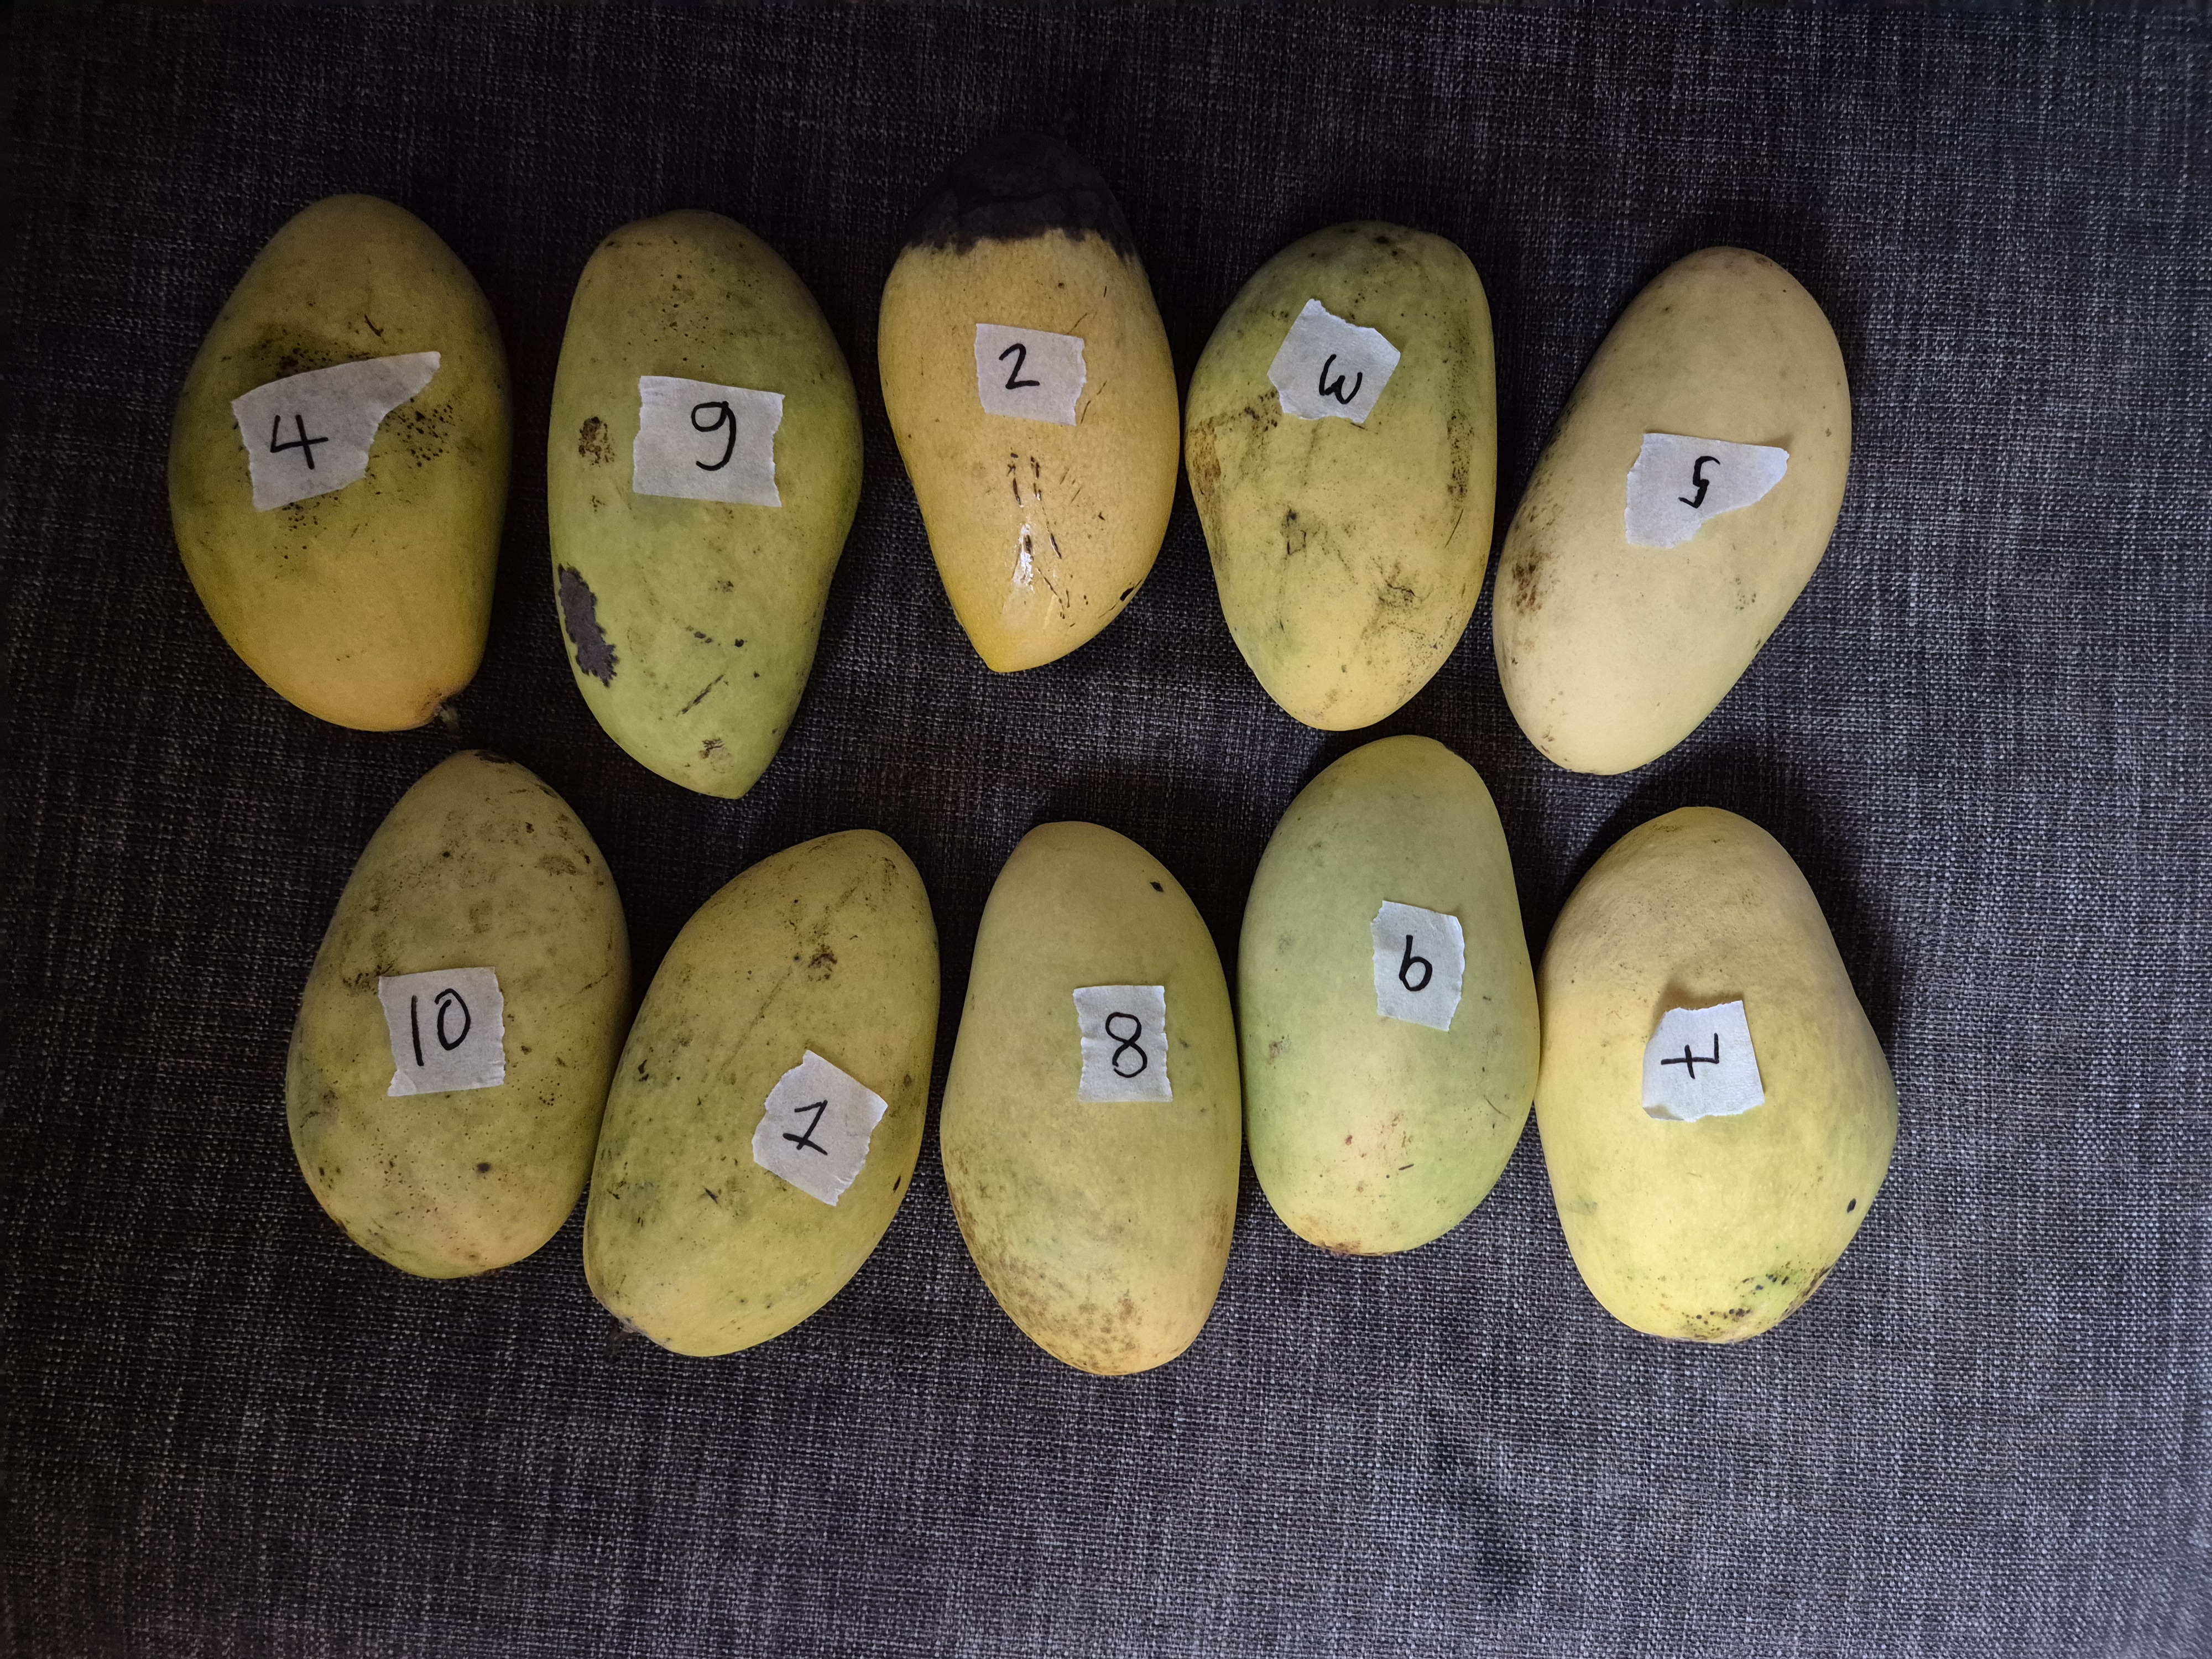
\includegraphics[width=0.45\textwidth]{/size-mango-test/ripe}
        \label{fig:ripe-mango}
    }
    \caption{Mangoes Tested for Size Measurement}
    \label{fig:mango_size_test}
\end{figure}

% \begin{figure}[!htbp]
%     \centering
%     \subbottom[Length Comparison in cm]{
%         \includegraphics[width=0.45\textwidth]{/size_new_graph/fig01}
%         \label{fig:length_cm}
%     }
%     \hfill
%     \subbottom[Width Comparison in cm]{
%         \includegraphics[width=0.45\textwidth]{/size_new_graph/fig02}
%         \label{fig:width_cm}
%     }
%     \caption{Predicted Length and Width for Both Methods}
%     \label{fig:length_and_width}
% \end{figure}

\begin{figure}[!htbp]
	\centering
	\includegraphics[width=1\textwidth]{/size_new_graph/fig01}
	\caption{Length Comparison in cm}
	\label{fig:length_cm}
\end{figure}
\begin{figure}[!htbp]
	\centering
	\includegraphics[width=1\textwidth]{/size_new_graph/fig02}
	\caption{Width Comparison in cm}
	\label{fig:width_cm}
\end{figure}

\begin{figure}[!htbp]
    \centering
    \subbottom[Absolute Difference for Length in cm]{
        \includegraphics[width=0.45\textwidth]{/size_new_graph/fig05}
        \label{fig:abs_length}
    }
    \hfill
    \subbottom[Absolute Difference for Width in cm]{
        \includegraphics[width=0.45\textwidth]{/size_new_graph/fig06}
        \label{fig:abs_width}
    }
    \vfill
    \subbottom[Percent Difference for Length]{
        \includegraphics[width=0.45\textwidth]{/size_new_graph/fig03}
        \label{fig:percent_diff_length}
    }
    \hfill
    \subbottom[Percent Difference for Width]{
        \includegraphics[width=0.45\textwidth]{/size_new_graph/fig04}
        \label{fig:percent_diff_width}
    }
    \caption{Percent and Absolute Difference between Both Methods}
    \label{fig:percent_absolute_diff}
\end{figure}

\begin{figure}[!htbp]
    \centering
    \subbottom[Sample 1]{
        \includegraphics[width=0.45\textwidth]{/rcnn-result/1}
        \label{fig:box1}
    }
    \hfill
    \subbottom[Sample 2]{
        \includegraphics[width=0.45\textwidth]{/rcnn-result/2}
        \label{fig:box2}
    }
    \vfill
    \subbottom[Sample 3]{
        \includegraphics[width=0.45\textwidth]{/rcnn-result/3}
        \label{fig:box3}
    }
    \hfill
    \subbottom[Sample 4]{
        \includegraphics[width=0.45\textwidth]{/rcnn-result/4}
        \label{fig:box4}
    }
    \caption{Resulting Bounding Boxes of the Mangoes}
    \label{fig:bounding_boxes}
\end{figure}

\section{Formula with User Priority } \label{sec:userPriorityFormula}
\gls{not:bprio} and \gls{not:rprio} and \gls{not:sprio} are the \gls{User Priority-Based Grading} for bruises, ripeness, and size of the Carabao mango. 
Furthermore, \gls{not:bpred} and \gls{not:rpred} and \gls{not:spred} are the machine learning's predictions for bruises, ripeness, and size of the Carabao mango.
The formula for the user priority is given by:
\begin{equation}
	\label{eq:userPriority}	
  \text{Mango Grade} = \ensuremath{b \left( P \right)  B\left( P \right) + r \left( P \right) R\left( P \right) + s \left( P \right) S\left( P \right)}
\end{equation}

\noindent The machine learning predictions are assigned the following numerical values:

\subsection{Ripeness Scores:}
\begin{align}
r(\text{yellow}) &= 1.0 \\
r(\text{yellow\_green}) &= 2.0 \\
r(\text{green}) &= 3.0
\end{align}

\subsection{Bruises Scores:}
\begin{align}
b(\text{bruised}) &= 1.0 \\
b(\text{unbruised}) &= 2.0
\end{align}

\subsection{Size Scores:}
\begin{align}
s(\text{small}) &= 1.0 \\
s(\text{medium}) &= 2.0 \\
s(\text{large}) &= 3.0
\end{align}

\begin{figure}[!htbp]
	\centering
	\includegraphics[width=0.8\textwidth]{/priority/bruises-only}
	\caption{Only Bruises as a None Zero Value}
	\label{fig:bruises-only-input}
\end{figure}

\begin{figure}[!htbp]
	\centering
	\includegraphics[width=0.8\textwidth]{/priority/ripeness-and-bruises-only}
	\caption{Only Ripeness and Bruises as a None Zero Value}
	\label{fig:ripeness-bruises-only-input}
\end{figure}

\begin{figure}[!htbp]
	\centering
	\includegraphics[width=0.8\textwidth]{/priority/ripeness-only}
	\caption{Only Ripeness as a None Zero Value}
	\label{fig:ripeness-only-input}
\end{figure}

\section{Physical Prototype} \label{sec:physicalPrototype}

Add pictures of the hardware prototype here with description

\begin{figure}[!htbp]
    \centering
    \subbottom[Prototype Top View]{
        \includegraphics[width=0.45\textwidth]{top_view}
        \label{fig:top_view}
    }
    \hfill
    \subbottom[Entrance Conveyor Belt View]{
        \includegraphics[width=0.45\textwidth]{side1}
        \label{fig:side1}
    }
    \vfill
    \subbottom[Side Conveyor Belt View]{
        \includegraphics[width=0.45\textwidth]{side2}
        \label{fig:side2}
    }
    \caption{Version 1 of the Prototype}
    \label{fig:v1_prototype}
\end{figure}

\begin{figure}[!htbp]
    \centering
    \subbottom[Prototype Main Hardware]{
        \includegraphics[width=0.45\textwidth]{schematic1}
        \label{fig:schematic1}
    }
    \hfill
    \subbottom[DC Motor and Pulley]{
        \includegraphics[width=0.45\textwidth]{DC_Motor_Pulley}
        \label{fig:dc_motor_pulley}
    }
    \vfill
    \subbottom[LED Lights and Camera Module]{
        \includegraphics[width=0.45\textwidth]{camera}
        \label{fig:camera}
    }
    \caption{Hardware View}
    \label{fig:hardware_view}
\end{figure}

\begin{figure}[!htbp]
    \centering
    \subbottom[Side View of Improved Prototype]{
        \includegraphics[width=0.45\textwidth]{new-side-view}
        \label{fig:new-side-view}
    }
    \hfill
    \subbottom[Top View of Improved Prototype]{
        \includegraphics[width=0.45\textwidth]{new-top-view}
        \label{fig:new-top-view}
    }
    \caption{Version 2: Improved Prototype}
    \label{fig:v2_prototype}
\end{figure}

\section{Software Application}

Show the raspberry pi app UI and demonstrate it here 

\begin{figure}[!htbp]
    \centering
    \subbottom[Version 1.1]{
        \includegraphics[width=0.45\textwidth]{UI_v1}
        \label{fig:ui_v1}
    }
    \hfill
    \subbottom[Version 1.2]{
        \includegraphics[width=0.45\textwidth]{UI_v2}
        \label{fig:ui_v2}
    }
    \vfill
    \subbottom[Version 1.3]{
        \includegraphics[width=0.45\textwidth]{UI_v3}
        \label{fig:ui_v3}
    }

    \caption{Version 1 of the RPi's User Interface}
    \label{fig:user_interface_v1}
\end{figure}

\begin{figure}[!htbp]
    \centering
    \subbottom[Version 2.1 with Background Image]{
        \includegraphics[width=0.45\textwidth]{/ui/ui-version1}
        \label{fig:app_v4}
    }
    \hfill
    \subbottom[Version 2.2 without Background Image]{
        \includegraphics[width=0.45\textwidth]{/ui/ui-version2}
        \label{fig:app_v5}
    }
    \caption{Version 2 of the RPi's User Interface}
    \label{fig:ui_main_v2}
\end{figure}

\begin{figure}[!htbp]
    \centering
    \subbottom[Version 1]{
        \includegraphics[width=0.45\textwidth]{sort_tree_1}
        \label{fig:sort_tree}
    }
    \hfill
    \subbottom[Version 2]{
        \includegraphics[width=0.45\textwidth]{sort_folder}
        \label{fig:sort_folder}
    }
    \vfill
    \subbottom[Version 3]{
        \includegraphics[width=0.45\textwidth]{sort_input_prior}
        \label{fig:input_folder_prior}
    }

    \caption{Mango Image Sorted}
    \label{fig:img_sorted}
\end{figure}

\begin{figure}[!htbp]
    \centering
    \subbottom[All Zero Error]{
        \includegraphics[width=0.45\textwidth]{/errors/all-zero}
        \label{fig:all-zero}
    }
    \hfill
    \subbottom[Input Error]{
        \includegraphics[width=0.45\textwidth]{/errors/input-error}
        \label{fig:input-error}
    }
    \vfill
    \subbottom[Null Button Error]{
        \includegraphics[width=0.45\textwidth]{/errors/null-button}
        \label{fig:null-button}
    }

    \caption{Error Messages}
    \label{fig:error-handel-1}
\end{figure}

\begin{figure}[!htbp]
    \centering
    \subbottom[Not Number at Conveyor Time]{
        \includegraphics[width=0.45\textwidth]{/errors/letter-time}
        \label{fig:letter-time}
    }
    \hfill
    \subbottom[Not Number at Priority]{
        \includegraphics[width=0.45\textwidth]{/errors/letter-priority}
        \label{fig:letter-priority}
    }
    \caption{Error message for Letter as Input}
    \label{fig:error-handel-2}
\end{figure}

\begin{figure}[!htbp]
	\centering
	\includegraphics[width=0.8\textwidth]{/ui/help}
	\caption{Help Page UI}
	\label{fig:help_page}
\end{figure}

\begin{figure}[!htbp]
    \centering
    \subbottom[Green and Unbruised]{
        \includegraphics[width=0.45\textwidth]{/ripe-class/green}
        \label{fig:green-result}
    }
    \hfill
    \subbottom[Yellow\_Green and Bruised]{
        \includegraphics[width=0.45\textwidth]{/ripe-class/yellow-green}
        \label{fig:yellow-green-result}
    }
    \vfill
    \subbottom[Yellow and Bruised]{
        \includegraphics[width=0.45\textwidth]{/ripe-class/yellow}
        \label{fig:yellow-result}
    }

    \caption{Sample Ripeness and Bruises Results}
    \label{fig:ripeness-all}
\end{figure}

\begin{lstlisting}[
float=h,
caption=More CNN Training Results for GPU, 
label=lst:more_cnn_training_gpu,
language=TeX,
frame=single]
Network            | Prec  | Rec   | F1    | Acc | Time    | VRAM
-------------------|-------|-------|-------|-----|---------|-----
VGG16              | 0.188 | 0.434 | 0.263 | 43  | 2h57m   | 7.0
ALEXNET            | 0.188 | 0.434 | 0.263 | 43  | 4h23m   | 2.3
RESNET50           | 0.870 | 0.869 | 0.868 | 87  | 7h13m   | 4.1
GOOGLENET          | 0.898 | 0.895 | 0.892 | 89  | 3h3m    | 2.9
MOBILENETV2        | 0.898 | 0.898 | 0.897 | 90  | 2h0m    | 3.6
DENSENET121        | 0.877 | 0.877 | 0.875 | 88  | 2h10m   | 5.5
EFFICIENTNET B0    | 0.890 | 0.888 | 0.887 | 89  | 2h26m   | 4.1
EFFICIENTNET B1    | 0.867 | 0.862 | 0.859 | 86  | 2h30m   | 5.3
EFFICIENTNET B2    | 0.927 | 0.924 | 0.925 | 92  | 2h14m   | 5.5
EFFICIENTNET B3    | 0.882 | 0.880 | 0.879 | 88  | 2h25m   | 6.8
EFFICIENTNET B4    | 0.899 | 0.898 | 0.896 | 90  | 2h50m   | 8.0
EFFICIENTNET B5    | 0.925 | 0.924 | 0.924 | 92  | 5h49m   | 11.6
EFFICIENTNET B6    | 0.934 | 0.933 | 0.933 | 93  | 7h51m   | 14.5
EFFICIENTNET B7    | 0.883 | 0.871 | 0.873 | 87  | 10h34m  | 18.8
EFFICIENTNETV2-B0  | 0.915 | 0.913 | 0.913 | 91  | 1h53m   | 3.0
EFFICIENTNETV2-B1  | 0.904 | 0.904 | 0.902 | 90  | 2h0m    | 3.6
EFFICIENTNETV2-B2  | 0.902 | 0.900 | 0.901 | 90  | 2h17m   | 3.8
EFFICIENTNETV2-B3  | 0.926 | 0.926 | 0.925 | 93  | 2h2m    | 4.5
EFFICIENTNETV2-S   | 0.894 | 0.893 | 0.891 | 89  | 1h59m   | 6.1
EFFICIENTNETV2-M   | 0.893 | 0.893 | 0.892 | 89  | 2h58m   | 9.9
EFFICIENTNETV2-L   | 0.875 | 0.871 | 0.870 | 87  | 14h58m  | 16.8
-------------------|-------|-------|-------|-----|---------|-----
AVERAGE            | 0.830 | 0.852 | 0.835 | 85  | -       | 7.0
\end{lstlisting} 

\begin{lstlisting}[
float=h,
caption=More CNN Training Results for CPU, 
label=lst:more_cnn_training_cpu,
language=TeX,
frame=single]
Network            | Prec  | Rec   | F1    | Acc | Time    | Mem
-------------------|-------|-------|-------|-----|---------|----
VGG16              | 0.297 | 0.545 | 0.384 | 54  | 5h38m   | 6.5
ALEXNET            | 0.297 | 0.545 | 0.384 | 54  | 4h25m   | 3.3
RESNET50           | 0.858 | 0.844 | 0.844 | 84  | 8h24m   | 5.4
GOOGLENET          | 0.843 | 0.808 | 0.799 | 81  | 3h14m   | 4.0
MOBILENETV2        | 0.859 | 0.858 | 0.858 | 86  | 3h44m   | 4.8
DENSENET121        | 0.839 | 0.838 | 0.838 | 84  | 3h8m    | 6.7
EFFICIENTNET B0    | 0.873 | 0.870 | 0.870 | 87  | 2h37m   | 5.3
EFFICIENTNET B1    | 0.898 | 0.897 | 0.896 | 90  | 3h8m    | 6.7
EFFICIENTNET B2    | 0.901 | 0.901 | 0.901 | 90  | 2h56m   | 6.7
EFFICIENTNET B3    | 0.913 | 0.913 | 0.913 | 91  | 3h27m   | 8.0
EFFICIENTNET B4    | 0.897 | 0.897 | 0.897 | 90  | 4h17m   | 9.8
EFFICIENTNET B5    | 0.892 | 0.883 | 0.881 | 88  | 5h45m   | 12.2
EFFICIENTNET B6    | 0.884 | 0.883 | 0.882 | 88  | 7h12m   | 14.5
EFFICIENTNET B7    | 0.857 | 0.856 | 0.856 | 86  | 9h9m    | 18.0
EFFICIENTNETV2-B0  | 0.873 | 0.860 | 0.858 | 86  | 2h6m    | 4.4
EFFICIENTNETV2-B1  | 0.893 | 0.893 | 0.893 | 89  | 3h30m   | 5.1
EFFICIENTNETV2-B2  | 0.888 | 0.881 | 0.881 | 88  | 2h45m   | 5.4
EFFICIENTNETV2-B3  | 0.905 | 0.905 | 0.905 | 90  | 2h32m   | 6.2
EFFICIENTNETV2-S   | 0.860 | 0.836 | 0.831 | 84  | 2h55m   | 7.7
EFFICIENTNETV2-M   | 0.856 | 0.846 | 0.846 | 85  | 2h37m   | 9.3
EFFICIENTNETV2-L   | 0.849 | 0.836 | 0.836 | 84  | 13h39m  | 17.9
-------------------|-------|-------|-------|-----|---------|----
AVERAGE            | 0.820 | 0.838 | 0.821 | 84  | -       | 8.0
\end{lstlisting} 

\begin{lstlisting}[
float=h,
caption=Mango Size Results, 
label=lst:more_size_results01,
language=TeX,
frame=single]
ID | Weight | Ground Truth | V2 Code    | V1 Code    
   | (g)    | L   | W      | L    | W   | L    | W    
---|--------|-----|--------|------|-----|------|------
01 | 260.8  | 11.8| 7.80   | 12.86| 7.96| 10.33| 3.08
02 | 299.4  | 12.8| 7.80   | 14.69| 8.30| 11.59| 3.73
03 | 238.4  | 11.4| 7.60   | 12.42| 7.60| 9.17 | 2.36
04 | 335.6  | 13.8| 10.50  | 15.38| 9.33| 12.49| 5.00
05 | 272.4  | 12.9| 8.50   | 15.13| 7.81| 11.52| 3.96
06 | 267.9  | 13.1| 8.20   | 15.72| 7.73| 11.78| 3.58
07 | 274.0  | 12.6| 8.20   | 14.96| 7.88| 11.80| 4.00
08 | 272.3  | 13.3| 8.00   | 15.56| 7.49| 12.02| 4.26
09 | 281.6  | 13.0| 8.00   | 15.20| 7.55| 12.12| 4.26
10 | 286.2  | 13.8| 8.00   | 15.20| 7.55| 12.17| 3.09
11 | 284.6  | 12.6| 9.00   | 15.20| 7.55| 10.90| 3.26
12 | 265.7  | 13.3| 8.00   | 14.80| 8.48| 11.38| 2.98
13 | 278.1  | 13.0| 7.60   | 15.08| 7.87| 11.00| 3.18
14 | 263.8  | 12.9| 7.50   | 15.11| 7.75| 11.28| 4.11
15 | 222.0  | 12.1| 7.80   | 12.96| 7.44| 10.73| 3.17
16 | 240.1  | 13.5| 8.20   | 15.36| 7.14| 11.15| 3.21
17 | 290.7  | 13.5| 8.50   | 14.71| 8.20| 11.76| 3.21
18 | 260.1  | 12.8| 8.00   | 14.52| 7.65| 10.91| 3.12
19 | 253.6  | 12.9| 7.50   | 14.08| 7.66| 11.65| 3.17
20 | 225.9  | 12.0| 7.50   | 13.17| 7.48| 10.49| 3.24
---|--------|-----|--------|------|-----|------|------
AVG| 264.1  | 12.8| 8.1    | 14.7 | 7.8 | 11.3 | 3.5
\end{lstlisting}

\begin{lstlisting}[
float=h,
caption=Mango Size Difference to Ground Truth Results, 
label=lst:more_size_results02,
language=TeX,
frame=single]
ID | V2 Difference | V1 Difference
   |  L   |   W    |  L   |   W   
---|------|--------|------|-------
01 | 1.06 |  0.16  | 1.47 |  4.72
02 | 1.89 |  0.50  | 1.21 |  4.07
03 | 1.02 |  0.00  | 2.23 |  5.24
04 | 1.58 |  1.17  | 1.31 |  5.50
05 | 2.23 |  0.69  | 1.38 |  4.54
06 | 2.62 |  0.47  | 1.32 |  4.62
07 | 2.36 |  0.32  | 0.80 |  4.20
08 | 2.26 |  0.51  | 1.28 |  3.74
09 | 2.20 |  0.45  | 1.12 |  3.74
10 | 1.40 |  0.45  | 1.63 |  4.91
11 | 2.60 |  1.45  | 1.70 |  5.74
12 | 1.50 |  0.48  | 1.92 |  5.02
13 | 2.08 |  0.27  | 2.00 |  4.42
14 | 2.21 |  0.25  | 1.62 |  3.39
15 | 0.86 |  0.36  | 1.37 |  4.63
16 | 1.86 |  1.06  | 2.35 |  4.99
17 | 1.21 |  0.30  | 1.74 |  5.29
18 | 1.72 |  0.35  | 1.89 |  4.88
19 | 1.18 |  0.16  | 1.25 |  4.33
20 | 1.17 |  0.02  | 1.51 |  4.26
---|------|--------|------|-------
AVG| 1.80 |  0.50  | 1.60 |  4.60
\end{lstlisting}

\begin{lstlisting}[
float=h,
caption=Mean and Standard Deviation of Size, 
label=lst:mean_and_std_results,
language=TeX,
frame=single]
Metric                    | V2 Code           | V1 Code
                          | Mean    | SD      | Mean    | SD
--------------------------|---------|---------|---------|--------
Length Differences (cm)   | 1.75    | 0.56    | 1.54    | 0.40
Width Differences (cm)    | 0.47    | 0.37    | 4.61    | 0.61
Length Percent Difference | 13.57%  | 4.20%   | 12.04%  | 3.28%
Width Percent Difference  | 3.24%   | 6.16%   | 56.89%  | 6.32%
\end{lstlisting}

\section{Summary} \label{sec:summary_results_and_discussions}

Provide the gist of this chapter such that it reflects the contents and the message. This is a compile test
\\


	%	\stopcontents[chapters]
	\cleardoublepage
	\fi
	
	%%%%%%%%%%%%%%%%%%%%%%%%%%%%%%%%%%%%%%%%%%%%%%%%
	\ifConc
	\chapter{Conclusions, Recommendations, and Future Directives} 
	\label{ch:conc} 
	%	\startcontents[chapters]
	%	\begin{SingleSpace}	
	%		\Mprintcontents 
	%	\end{SingleSpace}
		\section{Concluding Remarks}

In this \documentType, the prototype is successful in grading and sorting Carabao mangoes based on 
the user priority and machine learning algorithm. More specifically, the prototype is successful in
automatimcally classifying Carabao mangoes based on ripeness (Green, Green Yellow, and Yellow), 
size (Large, Medium, Small), and bruises (bruised and not bruised)

\section{Contributions}

The contributions of each group member are as follows:
\begin{itemize}
  \item BANAL Kenan A.: Scrum Master (Project manager in charge of the hardware and software integration) 
  \item BAUTISTA Francis Robert Miguel F.: Front End Engineer (UI/UX Designer in charge of software interface 
  and hardware assistant of the Scrum Master) 
  \item HERMOSURA Don Humphrey L. : Back End Engineer (Software Engineer in charge of the 
  machine learning algorithm and software assistant of the Scrum Master)
  \item SALAZAR Daniel G.: Product Engineer (Software Engineer in charge of training and testing of 
  the machine learning algorithm)
\end{itemize}


\section{Recommendations}

The researchers recommend that the prototype be improved in the optimization of the machine learning algorithm
and the hardware design. The researchers also recommend that the prototype be tested in the 
actual grading and sorting of Carabao mangoes in the market. 

\section{Future Prospects}

Future researchers may consider the following recommendations for future work:
\begin{enumerate}
	\item  User testing of the prototype in the actual grading and sorting of Carabao mangoes in the Philippine market.
	\item  Additional of weight measurement to the prototype to improve the grading and sorting of Carabao mangoes.
	\item  Integration of a custom PCB to improve the hardware design of the prototype.
\end{enumerate}


	%	\stopcontents[chapters]
	\cleardoublepage
	\fi
	
	%%%%%%%%%%%%%%%%%%%%%%%%%%%%%%%%%%%%%%%%%%%%%%%
	\renewcommand{\UrlFont}{\normalfont}
	%\bibliographystyle{IEEEtr} % for IEEE referencing format
	\bibliographystyle{apalike} % for APA referencing format
	\begin{SingleSpace}
		{\small \bibliography{references}}

		
	\end{SingleSpace}
	\vfill
	\begin{flushright}
		Produced: \usdate\today, \currenttime \\
	\end{flushright}
	\cleardoublepage 
	
	%%%%%%%%%%%%%%%%%%%%%%%%%%%%%%%%%%%%%%%%%%%%%%%%
	\SingleSpacing
	\appendix
	\renewcommand{\thechapter}{\Alph{chapter}}
	\renewcommand{\thesection}{\thechapter\arabic{section}}
	\appto\appendix{\renewcommand\thechapter{\AlphAlph{\value{chapter}}}} % for increasing appendix chapters beyond Z, i.e. AA, AB, etc.
	
	%%%%%%%%%%%%%%%%%%%%%%%%%%%%%%%%%%%%%%%%%%%%%%%%
	\chapter{Student Research Ethics Clearance}
	\includepdf[pages={1},%
	offset=3.5mm -10mm,%
	scale=0.75,%
	pagecommand={},]
	{./figure/STUDENT_RESEARCH_ETHICS_CLEARANCE.pdf}
	\cleardoublepage
	
	%%%%%%%%%%%%%%%%%%%%%%%%%%%%%%%%%%%%%%%%%%%%%%%%
	% \chapter{Answers to Questions to this \documentType}
	% %\startcontents[chapters]
	% %\Mprintcontents 
	% \include{answers_to_questions}
	% %\stopcontents[chapters]
	% \cleardoublepage
	
	%%%%%%%%%%%%%%%%%%%%%%%%%%%%%%%%%%%%%%%%%%%%%%%%
	\chapter{Revisions to the Proposal} 
	\label{ch:revisions_to_the_proposal}
	%\startcontents[chapters]
	%\Mprintcontents  
	%\include{revisions_to_the_proposal}
	\includepdf[pages={1-5},
	offset=3.5mm -10mm,%
	scale=0.75,%
	pagecommand={},
	]{./figure/AppendixZ.pdf} % Includes all pages (1 to 5)
	%\stopcontents[chapters]
	\cleardoublepage
	
  %%%%%%%%%%%%%%%%%%%%%%%%%%%%%%%%%%%%%%%%%%%%%%%%
	\chapter{Questionaire to the Expert} 
	\label{ch:questionaire_to_expert}
	%\startcontents[chapters]
	%\Mprintcontents  
	%\include{revisions_to_the_proposal}
	\includepdf[pages={1-10},
	offset=3.5mm -10mm,%
	scale=0.75,%
	pagecommand={},
	]{./figure/questions.pdf} % Includes all pages (1 to 5)
	%\stopcontents[chapters]
	\cleardoublepage
	%%%%%%%%%%%%%%%%%%%%%%%%%%%%%%%%%%%%%%%%%%%%%%%%
	% \chapter{Revisions to the Final} 
	% \label{ch:revisions_to_the_final}
	% %\startcontents[chapters]
	% %\Mprintcontents  
	% \include{revisions_to_the_final}
	% %\stopcontents[chapters]	
	% \cleardoublepage
	
	%%%%%%%%%%%%%%%%%%%%%%%%%%%%%%%%%%%%%%%%%%%%%%%%
	%\chapter{Usage Examples} 
	%\label{ch:usage_examples}
	%\startcontents[chapters]
	%\Mprintcontents  
	%\include{usage_examples}
	%\stopcontents[chapters]
	%\cleardoublepage
	
	%%%%%%%%%%%%%%%%%%%%%%%%%%%%%%%%%%%%%%%%%%%%%%%%
	\ifPubList
	\include{publication}
	\fi
	\cleardoublepage
	
	%%%%%%%%%%%%%%%%%%%%%%%%%%%%%%%%%%%%%%%%%%%%%%%%
	\ifVita
	\chapter{Vita}


\foreach \n in {1,...,\numberOfAuthors}{
	\vfill
	\includegraphics[width=0.2\columnwidth]{vita_photo}
	\documentAuthor{firstname\n} \ \documentAuthor{surname\n} \ is currently taking up his B.Sc. \degree \ studies.  He is passionate about software and hardware systems such as Vivado, Arduino, C, and Python.
	
	\vfill
}
	\fi
	\cleardoublepage
	
	%%%%%%%%%%%%%%%%%%%%%%%%%%%%%%%%%%%%%%%%%%%%%%%%
	\ifIndex
	\printindex
	\fi
	
	%%%%%%%%%%%%%%%%%%%%%%%%%%%%%%%%%%%%%%%%%%%%%%%%
	% \chapter{Article Paper(s)} 
	% \label{ch:article_paper}
	% \cleardoublepage
	% {
	% \ClearWallPaper
	% \includepdf[pages=-,%
	% scale=1.0,%
	% frame,%
	% ]
	% {article_forum_paper.pdf}
	% }
	% \cleardoublepage

\end{document}
